\documentclass[fleqn,10pt]{wlscirep}
\usepackage[utf8]{inputenc}
\usepackage{float}
\usepackage{fancyheadings}
\usepackage{amsmath}
\usepackage{amssymb}
\usepackage{graphicx}
\usepackage{booktabs}
\usepackage{tabularx}
\usepackage{lmodern}
\usepackage{outlines}
\usepackage{bm}
\usepackage{xr}
\usepackage{subfig}
\usepackage{algorithm,algpseudocode}
\usepackage{caption}
\usepackage{threeparttable}
\usepackage{multirow}
\usepackage{booktabs, tabularx}
\pagestyle{fancy}
\usepackage{pdflscape}
\usepackage{afterpage}
\usepackage{geometry}
\usepackage{color, colortbl}
\usepackage{xcolor}
\usepackage[T1]{fontenc}
\usepackage{lineno}
\usepackage[authoryear]{natbib}
\usepackage[normalem]{ulem}
\linenumbers

\title{Combining Human Expertise with Artificial Intelligence}

% omitting $\dag$
\author[1,]{Nikhil Agarwal}
\author[2]{Tan DT Bui}
\author[3]{Curtis P. Langlotz}
\author[4]{Matthew P. Lungren}
\author[5]{Alex Moehring}
\author[6]{Anuj Pareek}
\author[7]{Pranav Rajpurkar}
\author[1]{Tobias Salz}
\author[2]{Steven QH Truong}
\author[8]{Manasi Kutwal}
\affil[1]{MIT and NBER, Department of Economics, Cambridge, MA, 02142, United States}
\affil[2]{VinBrain, Hanoi, Vietnam}
\affil[3]{Stanford University, University Medical Line, Stanford, CA 94305, United States}
\affil[4]{Stanford University, Medical Center, Stanford, CA 94305, United States}
\affil[5]{MIT, Sloan School of Management, Cambridge, MA, 02142, United States}
\affil[6]{Stanford University, Center for Artificial Intelligence in Medicine \& Imaging, Stanford, CA 94304, United States}
\affil[7]{Harvard Medical School, Department of Biomedical Informatics, Cambridge, MA 02115, United States}
\affil[8]{MIT Economics, Blueprint Labs, Cambridge, MA, 02142, United States} 
%\affil[5]{Affiliation, department, city, postcode, country}
%\affil[*]{corresponding author(s): Derek Author (corresponding.author@email.example)}
%\affil[$\dag$]{these authors contributed equally to this work}


\begin{abstract}
%This is a manuscript template for Data Descriptor submissions to \emph{Scientific Data} (\href{http://www.nature.com/scientificdata}{http://www.nature.com/scientificdata}). The abstract must be no longer than 170 words, and should succinctly describe the study, the assay(s) performed, the resulting data, and the reuse potential, but should not make any claims regarding new scientific findings. No references are allowed in this section. 

Artificial Intelligence (AI) is often perceived to supplant humans in tasks requiring complex decision-making and reasoning. Contrary to this view, this dataset provides experimental data on human-AI collaboration to emphasize the need to study optimal collaboration between human experts and AI tools. Using a self-designed interface, we collect probabilistic assessments of $\sim$ 280 radiologists on a subset of 324 historical cases under various information and sequence settings. This paper provides insight into the purpose, collection approach, and example use cases of the dataset. The dataset can be used to understand the use of AI in medical diagnosis, and the dataset was used to study topics like how best to combine AI predictions with human input informed by contextual information and to understand potential human biases in using AI. Researchers can use this resource to explore questions regarding the use of AI in healthcare to improve diagnostic quality.
\end{abstract}

\begin{document}

\flushbottom
\maketitle
%  Click the title above to edit the author information and abstract

\thispagestyle{empty}

% \noindent Please note: Abbreviations should be introduced at the first mention in the main text – no abbreviations lists or tables should be included. 

\section*{Background \& Summary}

Advances in AI have raised concerns about the potential displacement of humans. While there is no doubt that AI has advanced enough to perform tasks requiring complex reasoning, machines still cannot perform the range of tasks that humans can \cite{Ng2016-nm}. In the context of radiology, while deep learning has improved precision in image recognition tasks, AI still cannot process clinical history information the way humans can. This complementarity of AI's precision and humans' contextual information necessitates the study of collaboration between these two. 

To study AI-human collaboration, we launched an experiment to collect chest X-ray diagnostic assessments for retrospective patient cases of $\sim280$ radiologists \footnote{Also referred to as participants, experts.} for 10 main thoracic pathologies (104 sub-pathologies conditional on the significant presence of main pathology) under different information conditions and design tracks. We acquired these assessments using a remote interface and through two modes: a) a continuous probabilistic value of pathology prevalence, and b) a  binarized recommendation on treatment/follow-up. 

The dataset contains additional information on time spent by radiologists on cases, clinical history information of the patients and values of two diagnostic standard specifications \footnote{Diagnostic standard is the indicative truth for the patient cases. We use this variable since a definitive diagnosis for most thoracic pathologies does not exist.} defined by the researchers. These diagnostic standard variables are derived from aggregating the assessments of five board-certified radiologists at Mt. Sinai Hospital and by estimating the leave-one-out mean of the probabilities reported by the radiologists in the experiment. 

Existing literature on this topic compares the performance of AI tools with human prediction power but does not explore how humans collaborate with AI. This dataset aims to fill the gap in the AI-expert collaboration field by providing an experimental and quantitative assessment of chest X-rays.

In the following sections, we discuss the summary statistics, example uses, variables, data collection, and augmentation that gives the resulting dataset. 


%(700 words maximum) An overview of the study design, the assay(s) performed, and the created data, including any background information needed to put this study in the context of previous work and the literature. The section should also briefly outline the broader goals that motivated the creation of this dataset and the potential reuse value. We also encourage authors to include a figure that provides a schematic overview of the study and assay(s) design. The Background \& Summary should not include subheadings. This section and the other main body sections of the manuscript should include citations to the literature as needed. 

\section*{Methods}

\subsection*{Data Collection}

The dataset was collected by researchers at the Massachusetts Institute of Technology (MIT) and Harvard University using a remote interface (Refer Appendix \ref{subsec:Appendix:-Experiment-Interface}). Participants for this experiment were recruited from teleradiology companies (first and third design) and the VinMac healthcare system in Vietnam (second design).

Of the 180 radiologists in the dataset, $\sim$17\% are US-based, and $\sim$20\% have a degree from the US. The average experience of radiologists in the dataset is 22 years, with $\sim$38\% working at large clinics. Of the 162 radiologists who responded to the sex question, 62\% are male. Close to 60\% of radiologists in the experiment had some or significant previous experience working with AI tools. 

The participating radiologists received randomized links to the experiment interface, which included training information, consent form, practice cases (only in designs 1 and 3), and the reads for data collection (Refer Appendix [subsec:Appendix:-Experiment-Interface]). The interface was designed to mimic the clinical setting for the participants. While we compensated the radiologists for participating in the experiment, we randomly provided monetary incentives to some radiologists in designs 1 and 3 \footnote{Participants in design 2 did not receive any monetary incentives because of the nature of the recruitment agreement.}.

During the experiment, we collected radiologists' diagnosis on patient cases across four different information environments:

\begin{enumerate}
    \item X-ray only
    \item X-ray with clinical history information
    \item X-ray with AI assistance 
    \item X-ray with AI assistance and clinical history information
\end{enumerate}

Different approaches to collecting this information had their advantages and disadvantages. Therefore, we create three distinct designs (visualized in figure \ref{fig:experiment_design}) to collect data on radiologists’ probabilities for the four information environments. Within each design, radiologists were randomized into different tracks (sequence of information environments). The proposed three hybrid designs collect both within and across subject data.

In each track, every radiologist views one of the 324 historical cases procured from the Stanford Healthcare System. These cases are manually reviewed for public release and contain X-ray and clinical history information. The use of retrospective cases allows us to avoid ethical and other issues that would arise when experimenting in high-stakes settings. For the AI assistance information environment, we provide radiologists with CheXpert, developed by a team of researchers at Stanford University \footnote{CheXpert is a deep learning algorithm trained on 224,316 chest radiographs of 65,240 patients and uses only the X-ray image to predict the prevalence of fourteen thoracic pathologies.}.

Finally, to establish the diagnostic standard for analyzing the quality of the radiologists' assessment, aggregate data on the assessments of five board-certified radiologists at Mt. Sinai hospital with at least ten years of experience and chest radiology as a sub-specialty was collected. In radiology, a definitive diagnostic standard is generally not available because of inherent variability in radiologists and their image-reading experience. We also introduce a diagnostic standard measure constructed using leave-one-out average of radiologists' assessments from the experiment. The reads used to calculate this diagnostic standard were from the treatment arm with clinical history but no AI assistance. Some other diagnostic standard variables in the dataset include the continuous diagnostic standard and the diagnostic standard constructed using log odds ratio. 

\subsubsection*{Designs}

\subsubsection*{Design 1}

In this design, we assign radiologists to a randomized sequence track (twenty-four tracks) of the four information environments. They read 15 patient cases, 60 in total, under every information environment. These cases are read sequentially without a repeat encounter. At the beginning of the experiment, every radiologist reads eight practice cases.

\subsubsection*{Design 2}

After the initial randomization at the track level into different information sequences, the radiologist read sixty patient cases per information environment and 240 cases in total. These cases are read over four sessions of sixty cases each, and every case is read under the four information environments. A minimum two-week washout period is introduced between each session to ensure that radiologists do not recall their/AI predictions from previous reads of the same case. Within every experiment session, 15 patient cases are read under every information environment in batches of 5, with no case repetition within a session.

\subsubsection*{Design 3}

The randomization in this design is based on access to clinical history in the first information environment versus not. To account for order effects from earlier in the experiment access to AI, the participants in this design receive AI access only after reading the same case in the XO or CH information environment. Radiologists diagnose the same 50 cases with and without assistance. Since the cases read with and without clinical history are different, they diagnose 100 cases in total.

\subsection*{Structure}

Every observation in the dataset refers to a radiologist-patient-pathology in a given experiment session. While there are no individual personal identifiers in the dataset, we have defined unique identifiers for each radiologist and patient-case used in the experiment. There is also information on the design type and the sequence in which each case was viewed by the radiologists within each experiment session. The major variables of interest in this dataset are: probability, treat, alg\_pred and the gt\_{*}{*} variables (refer to the variables list in Appendix \ref{subsec:Appendix:-Variables}) that include information collected using the remote interface. 

\subsection*{Data Summary \& Preliminary Analysis}

The following sections intend to discuss possible uses of the dataset
for future research. 

\subsubsection*{Summary Statistics}

In this section, we present some preliminary statistics on radiologists’ reported probability and decisions (table \ref{tab:summary_statistics}) and the effort exerted by the radiologists. The values have been reported across all the pre-registered groups: a) Top-level with AI, including the top-level pathologies of cardiomedistinal abnormality and airspace opacity. b) Pooled with AI, including all the pathologies with AI predictions while excluding abnormality and support device hardware. c) Pooled, including all pathologies with and without AI predictions. d) Abnormal, including cases marked as abnormal. As shown in the table \ref{tab:summary_statistics}, there is consistency in the reported statistics across the different designs.

In the experiment, for the top-level pathologies, the radiologists’ probability ranges from $\sim$0.21 to $\sim$0.25 across the three designs, with an average of 0.23. The low probability of treating a patient across the experiment points to the low prevalence rate of the pathologies considered. The radiologists make the correct decision approximately 70\% of the time, with radiologists from design 3 performing above average by 9\%. The average time spent by the radiologists on each case is $\sim$2.8 minutes, and the average across the designs ranges from 2.5 - 3 minutes. On average, the radiologists clicked 45 times when entering their predictions for each case. The measures of active time and clicks are relevant to study the effort exerted by the radiologists in the experiment.

The quality of the AI is assessed through the AI accuracy variable that measures the absolute deviation of the AI prediction from the diagnostic standard probability. For top-level and pooled with AI cases, the deviation is quite small, but the deviation is much larger for abnormal cases.
%0.56

\subsubsection*{Post experiment questionnaire}


At the end of the experiment, radiologists filled a survey based on their experience with the AI tool and clinical history used in making the assessments. These assessments are helpful in understanding the heterogeneity in radiologists’ qualities. Their responses allow the analysis of the extent to which AI and CH affect the assessment, decision-making and effort exerted in the diagnosis process. This information allows the exploration of questions across the quantitative assessments and qualitative beliefs.

AI influence (figure \ref{fig:ai-influence}): we try to evaluate the role played by AI in influencing radiologists actions. We find that while $\sim$45\% of radiologists agree that AI influences the assessment of a pathology's presence, only $\sim$28\% believe that it influences the diagnosis decision. Radiologists were split on their views of AI influencing their decision regarding follow-up treatment. This inconsistent treatment of AI signals by radiologists is important in understanding the costs faced by radiologists in integrating AI signals in decision-making. Consequently, one can study cognitive dissonance exhibited by the radiologists when it comes to using AI with the aid of this post-experiment questionnaire.

Clinical history influence (figure \ref{fig:ch-influence}): contrastingly, radiologists agreed to the influence of clinical history on all three fronts of assessment, decision-making and effort exertion. Clinical history is considered to be a critical component in diagnostic radiology, as it helps radiologists to narrow down to specific regions in the X-ray. Concurrently, its availability is believed to introduce cognitive biases like anchoring bias, attribution bias and framing bias (\cite{Yapp2022-tf}). Given these doubts about the benefits of clinical history, the radiologists’ probabilities and treatment decisions across different information environments in the dataset can be uses to study its importance. The radiologists in their answers to the question, "In what types of cases did the patient history matter?", frequently refer to certain conditions, as show in figure \ref{fig:ch-influence}. 

\section*{Data Records}

The Data Records section should be used to explain each data record associated with this work, including the repository where this information is stored, and to provide an overview of the data files and their formats. Each external data record should be cited numerically in the text of this section, for example \cite{Hao:gidmaps:2014}, and included in the main reference list as described below. A data citation should also be placed in the subsection of the Methods containing the data-collection or analytical procedure(s) used to derive the corresponding record. Providing a direct link to the dataset may also be helpful to readers (\hyperlink{https://doi.org/10.6084/m9.figshare.853801}{https://doi.org/10.6084/m9.figshare.853801}).

Tables should be used to support the data records, and should clearly indicate the samples and subjects (study inputs), their provenance, and the experimental manipulations performed on each (please see 'Tables' below). They should also specify the data output resulting from each data-collection or analytical step, should these form part of the archived record.

\section*{Technical Validation}

%This section presents any experiments or analyses that are needed to support the technical quality of the dataset. This section may be supported by figures and tables, as needed. This is a required section; authors must present information justifying the reliability of their data.

The code for the validation tasks can be found on the \href{https://github.com/mit-econ-ai/radiology_ai_data.}{GitHub repository}. 

\subsection*{Validation of diagnostic standard quality}

Here, we summarize evidence that the diagnostic standard we construct from the five board-certified radiologists from Mount Sinai, who each read all 324 patient cases in the study, is high quality and robust to various decisions an analyst could make. Table \ref{tab:diag_standard_quality} contains summary statistics for the ground truth created using the Mount Sinai radiologists and a leave-one- out internal ground truth calculated using the reads collected during the experiment under the treatment arm with clinical history but no AI assistance. Table \ref{tab:diag_standard_effort} contains additional summary statistics for the five Mount Sinai diagnostic standard labelers, including their average time and number of clicks. We also show the average agreement of the labels with the original radiologist’s read. Taken together, these analyses demonstrate, for the majority of cases, that the diagnostic standard labelers agree with the assessment of the radiologist who originally read the report in a clinical setting, and we can reject that the average probability assessment is equal to 0.5 at the 5% level.

\subsection*{Validation of radiologist read quality}

To benchmark the quality of AI predictions in our sample and the radiologists in our experiment, we compare our participant pool with the AI input using two performance measures in figure \ref{fig:compare_performance}. The first measure is derived from the receiver operating characteristic (ROC) curve, which measures the trade-off between the false positive and the true positive rate of a classifier as the cutoff for classifying a case as positive or negative is varied. It uses only ordinal information about the AI. A classifier that is not better than random has an AUROC value of 0.5 whereas a perfectly predictive classifier has a value of one. The second measure is the root mean squared error (RMSE), that utilizes cardinal information about the AI prediction. A lower RMSE indicates higher performance. We pool the data for top-level pathologies with AI for each radiologist’s reports and for the AI’s prediction.

\subsection*{Additional validation tests}

Additional validation tests can be found in the appendix of our NBER working paper, \cite{Agarwal2023-dn}. In the paper, we find that incentives do not play a significant role in a correct response. We also verify randomization occurred as expected through various balance and randomization tests. For design 2, we also find that the washout strategy was effective - radiologists’ predictions do not move towards the AI prediction if it was provided in a prior session but do if it is provided in the current session.

\section*{Usage Notes}

The dataset is hosted at XYZ link. Our \href{https://github.com/mit-econ-ai/radiology_ai_data}{GitHub repository} provides a detailed description and source code (Python scripts) on how to use this dataset and reproduce the published validation results. The data does not include any individual identifiers, although we do include our unique identifiers for each radiologist and patient-case. 

Using this dataset, one can answer questions such as: 1. How do humans/radiologists use AI assistance? 2. Is contextual information valuable? 3. Do the costs of AI-induced human biases outweigh the benefits? 4. What is the trade-off, if any, between the cost savings on human effort and decision-quality when delegating tasks to AI tools? 5. How do radiologists with different skill levels use AI assistance? These questions are indicative of the nature of research that can be undertaken with this data resource.

\subsection*{Usage for post-experiment questionnaire}

Some questions that can be explored using information from the post-experiment interview include: Do radiologists exert more effort and process information differently for these conditions compared to others? Does the mention of these conditions in the patient history indication affect the diagnosis? Is there consistency in what radiologists say in the post experiment questionnaire and what they actually end up doing? 


%The Usage Notes should contain brief instructions to assist other researchers with reuse of the data. This may include discussion of software packages that are suitable for analyzing the assay data files, suggested downstream processing steps (e.g. normalization, etc.), or tips for integrating or comparing the data records with other datasets. Authors are encouraged to provide code, programs or data-processing workflows if they may help others understand or use the data. Please see our code availability policy for advice on supplying custom code alongside Data Descriptor manuscripts.

%For studies involving privacy or safety controls on public access to the data, this section should describe in detail these controls, including how authors can apply to access the data, what criteria will be used to determine who may access the data, and any limitations on data use. 

\section*{Code availability}

Our \href{https://github.com/mit-econ-ai/radiology_ai_data}{GitHub repository} includes code (Python 3 and Stata 17) for

\begin{itemize}
    \item Data preparation
    \item Technical validation
    \item Summary statistics and post-experimental questionnaire
\end{itemize}

%For all studies using custom code in the generation or processing of datasets, a statement must be included under the heading "Code availability", indicating whether and how the code can be accessed, including any restrictions to access. This section should also include information on the versions of any software used, if relevant, and any specific variables or parameters used to generate, test, or process the current dataset. 

\nocite{*}
\bibliography{Datasheet.bib}

%\section*{Acknowledgements}  (not compulsory)

%Acknowledgements should be brief, and should not include thanks to anonymous referees and editors, or effusive comments. Grant or contribution numbers may be acknowledged.

\section*{Author contributions statement}

N.A. was responsible for 

%Must include all authors, identified by initials, for example: A.A. conceived the experiment(s), A.A. and B.A. conducted the experiment(s), C.A. and D.A. analysed the results. All authors reviewed the manuscript. 

\section*{Competing interests} 

The authors declare no competing interests.

%The corresponding author is responsible for providing a \href{https://www.nature.com/sdata/policies/editorial-and-publishing-policies#competing}{competing interests statement} on behalf of all authors of the paper. This statement must be included in the submitted article file.

\clearpage

\section*{Figures \& Tables}

\begin{figure}[ht]
    \centering
    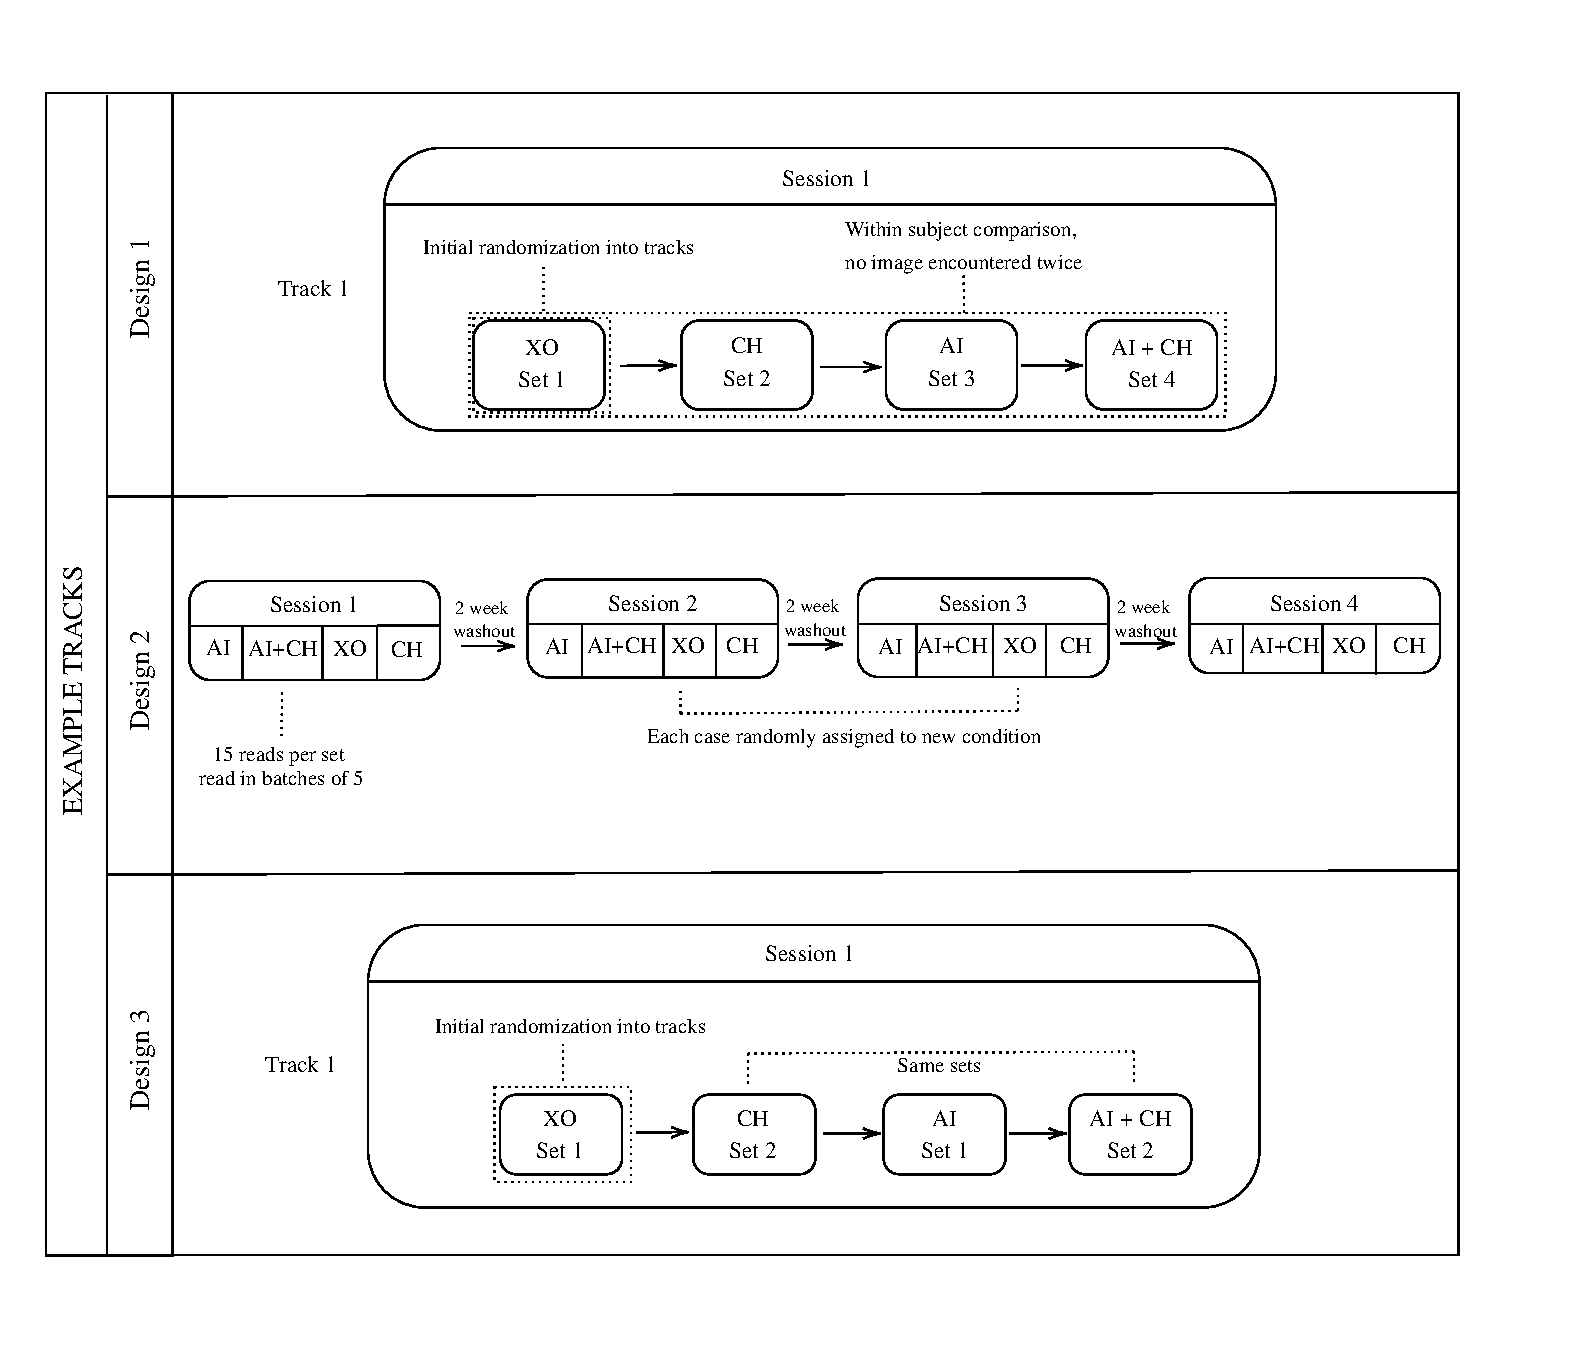
\includegraphics[width=0.8\textwidth]{images/designs.pdf}    
    \caption{Experimental designs}
    \label{fig:experiment_design}
\end{figure}

\begin{table}[ht]
    \centering
    \caption{Summary statistics\label{tab:summary_statistics}}
    \newcommand{\probtoplevelexpmean}{$0.233$}
\newcommand{\probtoplevelexpsd}{$0.290$}
\newcommand{\probtoplevelexpobs}{$36,280$}
\newcommand{\followuptoplevelexpmean}{$0.322$}
\newcommand{\followuptoplevelexpsd}{$0.467$}
\newcommand{\followuptoplevelexpobs}{$36,280$}
\newcommand{\devgttoplevelexpmean}{$0.223$}
\newcommand{\devgttoplevelexpsd}{$0.281$}
\newcommand{\devgttoplevelexpobs}{$36,280$}
\newcommand{\devaitoplevelexpmean}{$0.191$}
\newcommand{\devaitoplevelexpsd}{$0.169$}
\newcommand{\devaitoplevelexpobs}{$36,280$}
\newcommand{\aiaccuracytoplevelexpmean}{$0.261$}
\newcommand{\aiaccuracytoplevelexpsd}{$0.195$}
\newcommand{\aiaccuracytoplevelexpobs}{$36,280$}
\newcommand{\cordectoplevelexpmean}{$0.695$}
\newcommand{\cordectoplevelexpsd}{$0.460$}
\newcommand{\cordectoplevelexpobs}{$36,280$}
\newcommand{\activetimetoplevelexpmean}{$2.82$}
\newcommand{\activetimetoplevelexpsd}{$2.63$}
\newcommand{\activetimetoplevelexpobs}{$36,270$}
\newcommand{\clickstoplevelexpmean}{$45$}
\newcommand{\clickstoplevelexpsd}{$33$}
\newcommand{\clickstoplevelexpobs}{$36,270$}
\newcommand{\probradexpmean}{$0.250$}
\newcommand{\probradexpsd}{$0.304$}
\newcommand{\probradexpobs}{$180$}
\newcommand{\followupradexpmean}{$0.333$}
\newcommand{\followupradexpsd}{$0.473$}
\newcommand{\followupradexpobs}{$180$}
\newcommand{\devgtradexpmean}{$0.276$}
\newcommand{\devgtradexpsd}{$0.323$}
\newcommand{\devgtradexpobs}{$180$}
\newcommand{\devairadexpmean}{$0.205$}
\newcommand{\devairadexpsd}{$0.179$}
\newcommand{\devairadexpobs}{$180$}
\newcommand{\aiaccuracyradexpmean}{$0.281$}
\newcommand{\aiaccuracyradexpsd}{$0.215$}
\newcommand{\aiaccuracyradexpobs}{$180$}
\newcommand{\cordecradexpmean}{$0.678$}
\newcommand{\cordecradexpsd}{$0.469$}
\newcommand{\cordecradexpobs}{$180$}
\newcommand{\activetimeradexpmean}{$3.19$}
\newcommand{\activetimeradexpsd}{$3.24$}
\newcommand{\activetimeradexpobs}{$180$}
\newcommand{\clicksradexpmean}{$48$}
\newcommand{\clicksradexpsd}{$35$}
\newcommand{\clicksradexpobs}{$180$}
\newcommand{\probpooledaiexpmean}{$0.083$}
\newcommand{\probpooledaiexpsd}{$0.201$}
\newcommand{\probpooledaiexpobs}{$235,820$}
\newcommand{\followuppooledaiexpmean}{$0.122$}
\newcommand{\followuppooledaiexpsd}{$0.328$}
\newcommand{\followuppooledaiexpobs}{$235,820$}
\newcommand{\devgtpooledaiexpmean}{$0.085$}
\newcommand{\devgtpooledaiexpsd}{$0.205$}
\newcommand{\devgtpooledaiexpobs}{$235,820$}
\newcommand{\devaipooledaiexpmean}{$0.100$}
\newcommand{\devaipooledaiexpsd}{$0.135$}
\newcommand{\devaipooledaiexpobs}{$235,820$}
\newcommand{\aiaccuracypooledaiexpmean}{$0.117$}
\newcommand{\aiaccuracypooledaiexpsd}{$0.156$}
\newcommand{\aiaccuracypooledaiexpobs}{$235,820$}
\newcommand{\cordecpooledaiexpmean}{$0.882$}
\newcommand{\cordecpooledaiexpsd}{$0.323$}
\newcommand{\cordecpooledaiexpobs}{$235,820$}
\newcommand{\activetimepooledaiexpmean}{$2.82$}
\newcommand{\activetimepooledaiexpsd}{$2.63$}
\newcommand{\activetimepooledaiexpobs}{$235,755$}
\newcommand{\clickspooledaiexpmean}{$45$}
\newcommand{\clickspooledaiexpsd}{$33$}
\newcommand{\clickspooledaiexpobs}{$235,755$}
\newcommand{\probnormalexpmean}{$0.540$}
\newcommand{\probnormalexpsd}{$0.329$}
\newcommand{\probnormalexpobs}{$18,140$}
\newcommand{\followupnormalexpmean}{$0.528$}
\newcommand{\followupnormalexpsd}{$0.499$}
\newcommand{\followupnormalexpobs}{$18,140$}
\newcommand{\devgtnormalexpmean}{$0.423$}
\newcommand{\devgtnormalexpsd}{$0.323$}
\newcommand{\devgtnormalexpobs}{$18,140$}
\newcommand{\devainormalexpmean}{$0.245$}
\newcommand{\devainormalexpsd}{$0.204$}
\newcommand{\devainormalexpobs}{$18,140$}
\newcommand{\aiaccuracynormalexpmean}{$0.561$}
\newcommand{\aiaccuracynormalexpsd}{$0.279$}
\newcommand{\aiaccuracynormalexpobs}{$18,140$}
\newcommand{\cordecnormalexpmean}{$0.532$}
\newcommand{\cordecnormalexpsd}{$0.499$}
\newcommand{\cordecnormalexpobs}{$18,140$}
\newcommand{\activetimenormalexpmean}{$2.82$}
\newcommand{\activetimenormalexpsd}{$2.63$}
\newcommand{\activetimenormalexpobs}{$18,135$}
\newcommand{\clicksnormalexpmean}{$45$}
\newcommand{\clicksnormalexpsd}{$33$}
\newcommand{\clicksnormalexpobs}{$18,135$}
\newcommand{\probpooledexpmean}{$0.031$}
\newcommand{\probpooledexpsd}{$0.132$}
\newcommand{\probpooledexpobs}{$1,850,280$}
\newcommand{\followuppooledexpmean}{$0.077$}
\newcommand{\followuppooledexpsd}{$0.266$}
\newcommand{\followuppooledexpobs}{$526,060$}
\newcommand{\devgtpooledexpmean}{$0.032$}
\newcommand{\devgtpooledexpsd}{$0.133$}
\newcommand{\devgtpooledexpobs}{$1,850,280$}
\newcommand{\devaipooledexpmean}{$0.100$}
\newcommand{\devaipooledexpsd}{$0.135$}
\newcommand{\devaipooledexpobs}{$235,820$}
\newcommand{\aiaccuracypooledexpmean}{$0.117$}
\newcommand{\aiaccuracypooledexpsd}{$0.156$}
\newcommand{\aiaccuracypooledexpobs}{$235,820$}
\newcommand{\cordecpooledexpmean}{$0.979$}
\newcommand{\cordecpooledexpsd}{$0.144$}
\newcommand{\cordecpooledexpobs}{$1,850,280$}
\newcommand{\activetimepooledexpmean}{$2.82$}
\newcommand{\activetimepooledexpsd}{$2.63$}
\newcommand{\activetimepooledexpobs}{$1,849,770$}
\newcommand{\clickspooledexpmean}{$45$}
\newcommand{\clickspooledexpsd}{$33$}
\newcommand{\clickspooledexpobs}{$1,849,770$}

\newcommand{\probtopleveldomean}{$0.214$}
\newcommand{\probtopleveldosd}{$0.287$}
\newcommand{\probtopleveldoobs}{$13,440$}
\newcommand{\followuptopleveldomean}{$0.277$}
\newcommand{\followuptopleveldosd}{$0.448$}
\newcommand{\followuptopleveldoobs}{$13,440$}
\newcommand{\devgttopleveldomean}{$0.218$}
\newcommand{\devgttopleveldosd}{$0.290$}
\newcommand{\devgttopleveldoobs}{$13,440$}
\newcommand{\devaitopleveldomean}{$0.201$}
\newcommand{\devaitopleveldosd}{$0.171$}
\newcommand{\devaitopleveldoobs}{$13,440$}
\newcommand{\aiaccuracytopleveldomean}{$0.260$}
\newcommand{\aiaccuracytopleveldosd}{$0.193$}
\newcommand{\aiaccuracytopleveldoobs}{$13,440$}
\newcommand{\cordectopleveldomean}{$0.736$}
\newcommand{\cordectopleveldosd}{$0.441$}
\newcommand{\cordectopleveldoobs}{$13,440$}
\newcommand{\activetimetopleveldomean}{$3.03$}
\newcommand{\activetimetopleveldosd}{$3.17$}
\newcommand{\activetimetopleveldoobs}{$13,436$}
\newcommand{\clickstopleveldomean}{$43$}
\newcommand{\clickstopleveldosd}{$32$}
\newcommand{\clickstopleveldoobs}{$13,436$}
\newcommand{\probraddomean}{$0.180$}
\newcommand{\probraddosd}{$0.282$}
\newcommand{\probraddoobs}{$112$}
\newcommand{\followupraddomean}{$0.196$}
\newcommand{\followupraddosd}{$0.399$}
\newcommand{\followupraddoobs}{$112$}
\newcommand{\devgtraddomean}{$0.192$}
\newcommand{\devgtraddosd}{$0.295$}
\newcommand{\devgtraddoobs}{$112$}
\newcommand{\devairaddomean}{$0.174$}
\newcommand{\devairaddosd}{$0.164$}
\newcommand{\devairaddoobs}{$112$}
\newcommand{\aiaccuracyraddomean}{$0.234$}
\newcommand{\aiaccuracyraddosd}{$0.192$}
\newcommand{\aiaccuracyraddoobs}{$112$}
\newcommand{\cordecraddomean}{$0.830$}
\newcommand{\cordecraddosd}{$0.377$}
\newcommand{\cordecraddoobs}{$112$}
\newcommand{\activetimeraddomean}{$2.83$}
\newcommand{\activetimeraddosd}{$2.57$}
\newcommand{\activetimeraddoobs}{$112$}
\newcommand{\clicksraddomean}{$39$}
\newcommand{\clicksraddosd}{$26$}
\newcommand{\clicksraddoobs}{$112$}
\newcommand{\probpooledaidomean}{$0.074$}
\newcommand{\probpooledaidosd}{$0.194$}
\newcommand{\probpooledaidoobs}{$87,360$}
\newcommand{\followuppooledaidomean}{$0.101$}
\newcommand{\followuppooledaidosd}{$0.302$}
\newcommand{\followuppooledaidoobs}{$87,360$}
\newcommand{\devgtpooledaidomean}{$0.079$}
\newcommand{\devgtpooledaidosd}{$0.206$}
\newcommand{\devgtpooledaidoobs}{$87,360$}
\newcommand{\devaipooledaidomean}{$0.104$}
\newcommand{\devaipooledaidosd}{$0.137$}
\newcommand{\devaipooledaidoobs}{$87,360$}
\newcommand{\aiaccuracypooledaidomean}{$0.117$}
\newcommand{\aiaccuracypooledaidosd}{$0.155$}
\newcommand{\aiaccuracypooledaidoobs}{$87,360$}
\newcommand{\cordecpooledaidomean}{$0.901$}
\newcommand{\cordecpooledaidosd}{$0.299$}
\newcommand{\cordecpooledaidoobs}{$87,360$}
\newcommand{\activetimepooledaidomean}{$3.03$}
\newcommand{\activetimepooledaidosd}{$3.17$}
\newcommand{\activetimepooledaidoobs}{$87,334$}
\newcommand{\clickspooledaidomean}{$43$}
\newcommand{\clickspooledaidosd}{$32$}
\newcommand{\clickspooledaidoobs}{$87,334$}
\newcommand{\probnormaldomean}{$0.495$}
\newcommand{\probnormaldosd}{$0.324$}
\newcommand{\probnormaldoobs}{$6,720$}
\newcommand{\followupnormaldomean}{$0.526$}
\newcommand{\followupnormaldosd}{$0.499$}
\newcommand{\followupnormaldoobs}{$6,720$}
\newcommand{\devgtnormaldomean}{$0.400$}
\newcommand{\devgtnormaldosd}{$0.308$}
\newcommand{\devgtnormaldoobs}{$6,720$}
\newcommand{\devainormaldomean}{$0.277$}
\newcommand{\devainormaldosd}{$0.211$}
\newcommand{\devainormaldoobs}{$6,720$}
\newcommand{\aiaccuracynormaldomean}{$0.565$}
\newcommand{\aiaccuracynormaldosd}{$0.279$}
\newcommand{\aiaccuracynormaldoobs}{$6,720$}
\newcommand{\cordecnormaldomean}{$0.534$}
\newcommand{\cordecnormaldosd}{$0.499$}
\newcommand{\cordecnormaldoobs}{$6,720$}
\newcommand{\activetimenormaldomean}{$3.03$}
\newcommand{\activetimenormaldosd}{$3.17$}
\newcommand{\activetimenormaldoobs}{$6,718$}
\newcommand{\clicksnormaldomean}{$43$}
\newcommand{\clicksnormaldosd}{$32$}
\newcommand{\clicksnormaldoobs}{$6,718$}
\newcommand{\probpooleddomean}{$0.029$}
\newcommand{\probpooleddosd}{$0.127$}
\newcommand{\probpooleddoobs}{$685,440$}
\newcommand{\followuppooleddomean}{$0.066$}
\newcommand{\followuppooleddosd}{$0.247$}
\newcommand{\followuppooleddoobs}{$194,880$}
\newcommand{\devgtpooleddomean}{$0.030$}
\newcommand{\devgtpooleddosd}{$0.134$}
\newcommand{\devgtpooleddoobs}{$685,440$}
\newcommand{\devaipooleddomean}{$0.104$}
\newcommand{\devaipooleddosd}{$0.137$}
\newcommand{\devaipooleddoobs}{$87,360$}
\newcommand{\aiaccuracypooleddomean}{$0.117$}
\newcommand{\aiaccuracypooleddosd}{$0.155$}
\newcommand{\aiaccuracypooleddoobs}{$87,360$}
\newcommand{\cordecpooleddomean}{$0.982$}
\newcommand{\cordecpooleddosd}{$0.134$}
\newcommand{\cordecpooleddoobs}{$685,440$}
\newcommand{\activetimepooleddomean}{$3.03$}
\newcommand{\activetimepooleddosd}{$3.17$}
\newcommand{\activetimepooleddoobs}{$685,236$}
\newcommand{\clickspooleddomean}{$43$}
\newcommand{\clickspooleddosd}{$32$}
\newcommand{\clickspooleddoobs}{$685,236$}

\newcommand{\probtopleveltwmean}{$0.245$}
\newcommand{\probtopleveltwsd}{$0.278$}
\newcommand{\probtopleveltwobs}{$15,840$}
\newcommand{\followuptopleveltwmean}{$0.400$}
\newcommand{\followuptopleveltwsd}{$0.490$}
\newcommand{\followuptopleveltwobs}{$15,840$}
\newcommand{\devgttopleveltwmean}{$0.232$}
\newcommand{\devgttopleveltwsd}{$0.265$}
\newcommand{\devgttopleveltwobs}{$15,840$}
\newcommand{\devaitopleveltwmean}{$0.172$}
\newcommand{\devaitopleveltwsd}{$0.159$}
\newcommand{\devaitopleveltwobs}{$15,840$}
\newcommand{\aiaccuracytopleveltwmean}{$0.261$}
\newcommand{\aiaccuracytopleveltwsd}{$0.195$}
\newcommand{\aiaccuracytopleveltwobs}{$15,840$}
\newcommand{\cordectopleveltwmean}{$0.620$}
\newcommand{\cordectopleveltwsd}{$0.485$}
\newcommand{\cordectopleveltwobs}{$15,840$}
\newcommand{\activetimetopleveltwmean}{$2.76$}
\newcommand{\activetimetopleveltwsd}{$1.93$}
\newcommand{\activetimetopleveltwobs}{$15,834$}
\newcommand{\clickstopleveltwmean}{$49$}
\newcommand{\clickstopleveltwsd}{$30$}
\newcommand{\clickstopleveltwobs}{$15,834$}
\newcommand{\probradtwmean}{$0.188$}
\newcommand{\probradtwsd}{$0.261$}
\newcommand{\probradtwobs}{$33$}
\newcommand{\followupradtwmean}{$0.333$}
\newcommand{\followupradtwsd}{$0.479$}
\newcommand{\followupradtwobs}{$33$}
\newcommand{\devgtradtwmean}{$0.141$}
\newcommand{\devgtradtwsd}{$0.190$}
\newcommand{\devgtradtwobs}{$33$}
\newcommand{\devairadtwmean}{$0.138$}
\newcommand{\devairadtwsd}{$0.131$}
\newcommand{\devairadtwobs}{$33$}
\newcommand{\aiaccuracyradtwmean}{$0.214$}
\newcommand{\aiaccuracyradtwsd}{$0.152$}
\newcommand{\aiaccuracyradtwobs}{$33$}
\newcommand{\cordecradtwmean}{$0.758$}
\newcommand{\cordecradtwsd}{$0.435$}
\newcommand{\cordecradtwobs}{$33$}
\newcommand{\activetimeradtwmean}{$2.33$}
\newcommand{\activetimeradtwsd}{$1.32$}
\newcommand{\activetimeradtwobs}{$33$}
\newcommand{\clicksradtwmean}{$42$}
\newcommand{\clicksradtwsd}{$21$}
\newcommand{\clicksradtwobs}{$33$}
\newcommand{\probpooledaitwmean}{$0.090$}
\newcommand{\probpooledaitwsd}{$0.199$}
\newcommand{\probpooledaitwobs}{$102,960$}
\newcommand{\followuppooledaitwmean}{$0.154$}
\newcommand{\followuppooledaitwsd}{$0.361$}
\newcommand{\followuppooledaitwobs}{$102,960$}
\newcommand{\devgtpooledaitwmean}{$0.090$}
\newcommand{\devgtpooledaitwsd}{$0.199$}
\newcommand{\devgtpooledaitwobs}{$102,960$}
\newcommand{\devaipooledaitwmean}{$0.094$}
\newcommand{\devaipooledaitwsd}{$0.127$}
\newcommand{\devaipooledaitwobs}{$102,960$}
\newcommand{\aiaccuracypooledaitwmean}{$0.117$}
\newcommand{\aiaccuracypooledaitwsd}{$0.156$}
\newcommand{\aiaccuracypooledaitwobs}{$102,960$}
\newcommand{\cordecpooledaitwmean}{$0.853$}
\newcommand{\cordecpooledaitwsd}{$0.354$}
\newcommand{\cordecpooledaitwobs}{$102,960$}
\newcommand{\activetimepooledaitwmean}{$2.76$}
\newcommand{\activetimepooledaitwsd}{$1.93$}
\newcommand{\activetimepooledaitwobs}{$102,921$}
\newcommand{\clickspooledaitwmean}{$49$}
\newcommand{\clickspooledaitwsd}{$30$}
\newcommand{\clickspooledaitwobs}{$102,921$}
\newcommand{\probnormaltwmean}{$0.603$}
\newcommand{\probnormaltwsd}{$0.310$}
\newcommand{\probnormaltwobs}{$7,920$}
\newcommand{\followupnormaltwmean}{$0.566$}
\newcommand{\followupnormaltwsd}{$0.496$}
\newcommand{\followupnormaltwobs}{$7,920$}
\newcommand{\devgtnormaltwmean}{$0.464$}
\newcommand{\devgtnormaltwsd}{$0.325$}
\newcommand{\devgtnormaltwobs}{$7,920$}
\newcommand{\devainormaltwmean}{$0.195$}
\newcommand{\devainormaltwsd}{$0.174$}
\newcommand{\devainormaltwobs}{$7,920$}
\newcommand{\aiaccuracynormaltwmean}{$0.559$}
\newcommand{\aiaccuracynormaltwsd}{$0.280$}
\newcommand{\aiaccuracynormaltwobs}{$7,920$}
\newcommand{\cordecnormaltwmean}{$0.487$}
\newcommand{\cordecnormaltwsd}{$0.500$}
\newcommand{\cordecnormaltwobs}{$7,920$}
\newcommand{\activetimenormaltwmean}{$2.76$}
\newcommand{\activetimenormaltwsd}{$1.93$}
\newcommand{\activetimenormaltwobs}{$7,917$}
\newcommand{\clicksnormaltwmean}{$49$}
\newcommand{\clicksnormaltwsd}{$30$}
\newcommand{\clicksnormaltwobs}{$7,917$}
\newcommand{\probpooledtwmean}{$0.034$}
\newcommand{\probpooledtwsd}{$0.132$}
\newcommand{\probpooledtwobs}{$807,840$}
\newcommand{\followuppooledtwmean}{$0.096$}
\newcommand{\followuppooledtwsd}{$0.294$}
\newcommand{\followuppooledtwobs}{$229,680$}
\newcommand{\devgtpooledtwmean}{$0.034$}
\newcommand{\devgtpooledtwsd}{$0.130$}
\newcommand{\devgtpooledtwobs}{$807,840$}
\newcommand{\devaipooledtwmean}{$0.094$}
\newcommand{\devaipooledtwsd}{$0.127$}
\newcommand{\devaipooledtwobs}{$102,960$}
\newcommand{\aiaccuracypooledtwmean}{$0.117$}
\newcommand{\aiaccuracypooledtwsd}{$0.156$}
\newcommand{\aiaccuracypooledtwobs}{$102,960$}
\newcommand{\cordecpooledtwmean}{$0.974$}
\newcommand{\cordecpooledtwsd}{$0.160$}
\newcommand{\cordecpooledtwobs}{$807,840$}
\newcommand{\activetimepooledtwmean}{$2.76$}
\newcommand{\activetimepooledtwsd}{$1.93$}
\newcommand{\activetimepooledtwobs}{$807,534$}
\newcommand{\clickspooledtwmean}{$49$}
\newcommand{\clickspooledtwsd}{$30$}
\newcommand{\clickspooledtwobs}{$807,534$}

\newcommand{\probtoplevelthmean}{$0.240$}
\newcommand{\probtoplevelthsd}{$0.322$}
\newcommand{\probtoplevelthobs}{$7,000$}
\newcommand{\followuptoplevelthmean}{$0.231$}
\newcommand{\followuptoplevelthsd}{$0.421$}
\newcommand{\followuptoplevelthobs}{$7,000$}
\newcommand{\devgttoplevelthmean}{$0.212$}
\newcommand{\devgttoplevelthsd}{$0.297$}
\newcommand{\devgttoplevelthobs}{$7,000$}
\newcommand{\devaitoplevelthmean}{$0.216$}
\newcommand{\devaitoplevelthsd}{$0.182$}
\newcommand{\devaitoplevelthobs}{$7,000$}
\newcommand{\aiaccuracytoplevelthmean}{$0.260$}
\newcommand{\aiaccuracytoplevelthsd}{$0.196$}
\newcommand{\aiaccuracytoplevelthobs}{$7,000$}
\newcommand{\cordectoplevelthmean}{$0.785$}
\newcommand{\cordectoplevelthsd}{$0.411$}
\newcommand{\cordectoplevelthobs}{$7,000$}
\newcommand{\activetimetoplevelthmean}{$2.58$}
\newcommand{\activetimetoplevelthsd}{$2.80$}
\newcommand{\activetimetoplevelthobs}{$7,000$}
\newcommand{\clickstoplevelthmean}{$42$}
\newcommand{\clickstoplevelthsd}{$39$}
\newcommand{\clickstoplevelthobs}{$7,000$}
\newcommand{\probradthmean}{$0.232$}
\newcommand{\probradthsd}{$0.319$}
\newcommand{\probradthobs}{$35$}
\newcommand{\followupradthmean}{$0.200$}
\newcommand{\followupradthsd}{$0.406$}
\newcommand{\followupradthobs}{$35$}
\newcommand{\devgtradthmean}{$0.150$}
\newcommand{\devgtradthsd}{$0.223$}
\newcommand{\devgtradthobs}{$35$}
\newcommand{\devairadthmean}{$0.212$}
\newcommand{\devairadthsd}{$0.180$}
\newcommand{\devairadthobs}{$35$}
\newcommand{\aiaccuracyradthmean}{$0.258$}
\newcommand{\aiaccuracyradthsd}{$0.193$}
\newcommand{\aiaccuracyradthobs}{$35$}
\newcommand{\cordecradthmean}{$0.829$}
\newcommand{\cordecradthsd}{$0.382$}
\newcommand{\cordecradthobs}{$35$}
\newcommand{\activetimeradthmean}{$2.52$}
\newcommand{\activetimeradthsd}{$2.53$}
\newcommand{\activetimeradthobs}{$35$}
\newcommand{\clicksradthmean}{$41$}
\newcommand{\clicksradthsd}{$33$}
\newcommand{\clicksradthobs}{$35$}
\newcommand{\probpooledaithmean}{$0.085$}
\newcommand{\probpooledaithsd}{$0.218$}
\newcommand{\probpooledaithobs}{$45,500$}
\newcommand{\followuppooledaithmean}{$0.092$}
\newcommand{\followuppooledaithsd}{$0.289$}
\newcommand{\followuppooledaithobs}{$45,500$}
\newcommand{\devgtpooledaithmean}{$0.083$}
\newcommand{\devgtpooledaithsd}{$0.215$}
\newcommand{\devgtpooledaithobs}{$45,500$}
\newcommand{\devaipooledaithmean}{$0.110$}
\newcommand{\devaipooledaithsd}{$0.147$}
\newcommand{\devaipooledaithobs}{$45,500$}
\newcommand{\aiaccuracypooledaithmean}{$0.117$}
\newcommand{\aiaccuracypooledaithsd}{$0.156$}
\newcommand{\aiaccuracypooledaithobs}{$45,500$}
\newcommand{\cordecpooledaithmean}{$0.911$}
\newcommand{\cordecpooledaithsd}{$0.284$}
\newcommand{\cordecpooledaithobs}{$45,500$}
\newcommand{\activetimepooledaithmean}{$2.58$}
\newcommand{\activetimepooledaithsd}{$2.80$}
\newcommand{\activetimepooledaithobs}{$45,500$}
\newcommand{\clickspooledaithmean}{$42$}
\newcommand{\clickspooledaithsd}{$39$}
\newcommand{\clickspooledaithobs}{$45,500$}
\newcommand{\probnormalthmean}{$0.484$}
\newcommand{\probnormalthsd}{$0.356$}
\newcommand{\probnormalthobs}{$3,500$}
\newcommand{\followupnormalthmean}{$0.445$}
\newcommand{\followupnormalthsd}{$0.497$}
\newcommand{\followupnormalthobs}{$3,500$}
\newcommand{\devgtnormalthmean}{$0.372$}
\newcommand{\devgtnormalthsd}{$0.333$}
\newcommand{\devgtnormalthobs}{$3,500$}
\newcommand{\devainormalthmean}{$0.298$}
\newcommand{\devainormalthsd}{$0.226$}
\newcommand{\devainormalthobs}{$3,500$}
\newcommand{\aiaccuracynormalthmean}{$0.559$}
\newcommand{\aiaccuracynormalthsd}{$0.279$}
\newcommand{\aiaccuracynormalthobs}{$3,500$}
\newcommand{\cordecnormalthmean}{$0.630$}
\newcommand{\cordecnormalthsd}{$0.483$}
\newcommand{\cordecnormalthobs}{$3,500$}
\newcommand{\activetimenormalthmean}{$2.58$}
\newcommand{\activetimenormalthsd}{$2.80$}
\newcommand{\activetimenormalthobs}{$3,500$}
\newcommand{\clicksnormalthmean}{$42$}
\newcommand{\clicksnormalthsd}{$39$}
\newcommand{\clicksnormalthobs}{$3,500$}
\newcommand{\probpooledthmean}{$0.031$}
\newcommand{\probpooledthsd}{$0.141$}
\newcommand{\probpooledthobs}{$357,000$}
\newcommand{\followuppooledthmean}{$0.054$}
\newcommand{\followuppooledthsd}{$0.226$}
\newcommand{\followuppooledthobs}{$101,500$}
\newcommand{\devgtpooledthmean}{$0.030$}
\newcommand{\devgtpooledthsd}{$0.138$}
\newcommand{\devgtpooledthobs}{$357,000$}
\newcommand{\devaipooledthmean}{$0.110$}
\newcommand{\devaipooledthsd}{$0.147$}
\newcommand{\devaipooledthobs}{$45,500$}
\newcommand{\aiaccuracypooledthmean}{$0.117$}
\newcommand{\aiaccuracypooledthsd}{$0.156$}
\newcommand{\aiaccuracypooledthobs}{$45,500$}
\newcommand{\cordecpooledthmean}{$0.985$}
\newcommand{\cordecpooledthsd}{$0.122$}
\newcommand{\cordecpooledthobs}{$357,000$}
\newcommand{\activetimepooledthmean}{$2.58$}
\newcommand{\activetimepooledthsd}{$2.80$}
\newcommand{\activetimepooledthobs}{$357,000$}
\newcommand{\clickspooledthmean}{$42$}
\newcommand{\clickspooledthsd}{$39$}
\newcommand{\clickspooledthobs}{$357,000$}


\small	
\begin{threeparttable}
\resizebox{.5\paperheight}{!}{%
\begin{tabular}{lcccccccc}

\toprule[2.3pt]
& \multicolumn{2}{c}{\textbf{Top-Level}} & \multicolumn{2}{c}{\textbf{Pooled}} & \multicolumn{2}{c}{\textbf{Pooled}} & \multicolumn{2}{c}{\textbf{Abnormal}} \\

& \multicolumn{2}{c}{\textbf{with AI}} & \multicolumn{2}{c}{\textbf{with AI}} &  &  &  &  \\

& Mean & SD & Mean & SD & Mean & SD & Mean & SD \\
\midrule 

& \multicolumn{8}{c}{\textsc{Panel A}: Pooled (Radiologists: \probradexpobs)} \\
\addlinespace

Reported Probability & \probtoplevelexpmean & \probtoplevelexpsd & \probpooledaiexpmean & \probpooledaiexpsd & \probpooledexpmean & \probpooledexpsd & \probnormalexpmean & \probnormalexpsd \\
\addlinespace

Decision: Treat & \followuptoplevelexpmean & \followuptoplevelexpsd & \followuppooledaiexpmean & \followuppooledaiexpsd & \followuppooledexpmean & \followuppooledexpsd & \followupnormalexpmean & \followupnormalexpsd \\
\addlinespace

Correct Decision & \cordectoplevelexpmean & \cordectoplevelexpsd & \cordecpooledaiexpmean & \cordecpooledaiexpsd & \cordecpooledexpmean & \cordecpooledexpsd & \cordecnormalexpmean & \cordecnormalexpsd \\
\addlinespace

Active time & \activetimetoplevelexpmean & \activetimetoplevelexpsd & \activetimepooledaiexpmean & \activetimepooledaiexpsd & \activetimepooledexpmean & \activetimepooledexpsd & \activetimenormalexpmean & \activetimenormalexpsd \\
\addlinespace

Number of Clicks & \clickstoplevelexpmean & \clickstoplevelexpsd & \clickspooledaiexpmean & \clickspooledaiexpsd & \clickspooledexpmean & \clickspooledexpsd & \clicksnormalexpmean & \clicksnormalexpsd \\
\addlinespace

AI Accuracy & \aiaccuracytoplevelexpmean & \aiaccuracytoplevelexpsd & \aiaccuracypooledaiexpmean & \aiaccuracypooledaiexpsd & - & - & \aiaccuracynormalexpmean & \aiaccuracynormalexpsd \\
\addlinespace

Observations & \multicolumn{2}{c}{\probtoplevelexpobs} & \multicolumn{2}{c}{\probpooledaiexpobs} & \multicolumn{2}{c}{\probpooledexpobs} & \multicolumn{2}{c}{\probnormalexpobs} \\

\addlinespace
\addlinespace


& \multicolumn{8}{c}{\textsc{Panel B}: Design 1 (Radiologists: \probraddoobs)} \\
\addlinespace

Reported Probability & \probtopleveldomean & \probtopleveldosd & \probpooledaidomean & \probpooledaidosd & \probpooleddomean & \probpooleddosd & \probnormaldomean & \probnormaldosd \\
\addlinespace

Decision: Treat & \followuptopleveldomean & \followuptopleveldosd & \followuppooledaidomean & \followuppooledaidosd & \followuppooleddomean & \followuppooleddosd & \followupnormaldomean & \followupnormaldosd \\
\addlinespace

Correct Decision & \cordectopleveldomean & \cordectopleveldosd & \cordecpooledaidomean & \cordecpooledaidosd & \cordecpooleddomean & \cordecpooleddosd & \cordecnormaldomean & \cordecnormaldosd \\
\addlinespace

Active time & \activetimetopleveldomean & \activetimetopleveldosd & \activetimepooledaidomean & \activetimepooledaidosd & \activetimepooleddomean & \activetimepooleddosd & \activetimenormaldomean & \activetimenormaldosd \\
\addlinespace

Number of Clicks & \clickstopleveldomean & \clickstopleveldosd & \clickspooledaidomean & \clickspooledaidosd & \clickspooleddomean & \clickspooleddosd & \clicksnormaldomean & \clicksnormaldosd \\
\addlinespace

Observations & \multicolumn{2}{c}{\probtopleveldoobs} & \multicolumn{2}{c}{\probpooledaidoobs} & \multicolumn{2}{c}{\probpooleddoobs} & \multicolumn{2}{c}{\probnormaldoobs} \\

\addlinespace
\addlinespace


& \multicolumn{8}{c}{\textsc{Panel C}: Design 2 (Radiologists: \probradtwobs)} \\
\addlinespace

Reported Probability & \probtopleveltwmean & \probtopleveltwsd & \probpooledaitwmean & \probpooledaitwsd & \probpooledtwmean & \probpooledtwsd & \probnormaltwmean & \probnormaltwsd \\
\addlinespace

Decision: Treat & \followuptopleveltwmean & \followuptopleveltwsd & \followuppooledaitwmean & \followuppooledaitwsd & \followuppooledtwmean & \followuppooledtwsd & \followupnormaltwmean & \followupnormaltwsd \\
\addlinespace

Correct Decision & \cordectopleveltwmean & \cordectopleveltwsd & \cordecpooledaitwmean & \cordecpooledaitwsd & \cordecpooledtwmean & \cordecpooledtwsd & \cordecnormaltwmean & \cordecnormaltwsd \\
\addlinespace

Active time & \activetimetopleveltwmean & \activetimetopleveltwsd & \activetimepooledaitwmean & \activetimepooledaitwsd & \activetimepooledtwmean & \activetimepooledtwsd & \activetimenormaltwmean & \activetimenormaltwsd \\
\addlinespace

Number of Clicks & \clickstopleveltwmean & \clickstopleveltwsd & \clickspooledaitwmean & \clickspooledaitwsd & \clickspooledtwmean & \clickspooledtwsd & \clicksnormaltwmean & \clicksnormaltwsd \\
\addlinespace

Observations & \multicolumn{2}{c}{\probtopleveltwobs} & \multicolumn{2}{c}{\probpooledaitwobs} & \multicolumn{2}{c}{\probpooledtwobs} & \multicolumn{2}{c}{\probnormaltwobs} \\

\addlinespace
\addlinespace

& \multicolumn{8}{c}{\textsc{Panel D}: Design 3 (Radiologists: \probradthobs)} \\
\addlinespace

Reported Probability & \probtoplevelthmean & \probtoplevelthsd & \probpooledaithmean & \probpooledaithsd & \probpooledthmean & \probpooledthsd & \probnormalthmean & \probnormalthsd \\
\addlinespace

Decision: Treat & \followuptoplevelthmean & \followuptoplevelthsd & \followuppooledaithmean & \followuppooledaithsd & \followuppooledthmean & \followuppooledthsd & \followupnormalthmean & \followupnormalthsd \\
\addlinespace

Correct Decision & \cordectoplevelthmean & \cordectoplevelthsd & \cordecpooledaithmean & \cordecpooledaithsd & \cordecpooledthmean & \cordecpooledthsd & \cordecnormalthmean & \cordecnormalthsd \\
\addlinespace

Active time & \activetimetoplevelthmean & \activetimetoplevelthsd & \activetimepooledaithmean & \activetimepooledaithsd & \activetimepooledthmean & \activetimepooledthsd & \activetimenormalthmean & \activetimenormalthsd \\
\addlinespace

Number of Clicks & \clickstoplevelthmean & \clickstoplevelthsd & \clickspooledaithmean & \clickspooledaithsd & \clickspooledthmean & \clickspooledthsd & \clicksnormalthmean & \clicksnormalthsd \\
\addlinespace

Observations & \multicolumn{2}{c}{\probtoplevelthobs} & \multicolumn{2}{c}{\probpooledaithobs} & \multicolumn{2}{c}{\probpooledthobs} & \multicolumn{2}{c}{\probnormalthobs} \\

\addlinespace
\addlinespace

\bottomrule[2.3pt]

\addlinespace
\end{tabular}%
}
\end{threeparttable}

    \noindent\begin{minipage}[t]{1\columnwidth}%
    {\scriptsize{}Note: This table presents summary statistics of the
    experimental data. The first panel pools across all three designs
    and the remaining three panels separate for each of the three designs
    respectively. Decision is an indicator for whether treatment/follow-up
    is recommended, correct decision is an indicator for whether the decision
    matches the diagnostic standard, deviation from diagnostic standard is the absolute
    difference between the reported probability and the diagnostic standard,
    deviation from AI is the absolute difference between the expert's
    reported probability and the AI's reported probability, active time
    is measured in minutes.}%
    \end{minipage}
\end{table}

\begin{table}[H]
    \centering
    \caption{Diagnostic Standard Quality}
    \begin{tabular}{lcccccc}
\toprule
 & \multicolumn{2}{c}{Prevalence} & \multicolumn{2}{c}{Share Rejecting 0.5} & \multicolumn{2}{c}{Average Number of Rads} \\
 & Sinai & Experiment & Sinai & Experiment & Sinai & Experiment \\
\midrule
Top-Level with AI & 0.147 & 0.125 & 0.696 & 0.775 & 5.00 & 14.04 \\
Pooled with AI & 0.043 & 0.031 & 0.892 & 0.932 & 5.00 & 14.04 \\
Abnormal & 0.194 & 0.525 & 0.583 & 0.568 & 5.00 & 14.04 \\
All Pathologies & 0.013 & 0.010 & 0.953 & 0.977 & 5.00 & 14.04 \\
\bottomrule
\end{tabular}

    \label{tab:diag_standard_quality}
    \noindent\begin{minipage}[t]{1\columnwidth}%
    {\scriptsize{}Note: For each of the pre-registered pathology groups, this table shows the average prevalence, the share of cases where we can reject that $\sum_{r=1}^{R}\frac{\pi_{r}(\omega_{i}=1|s_{i,r}^{E})}{R}=0.5$ at the 5\% level, and the average number of reads per case for both the Mount Sinai ground truth diagnostic standard labels and the experiment leave-one-out ground truth diagnostic standard.}%
    \end{minipage}
\end{table}

\begin{table}[H]
    \centering
    \caption{Diagnostic Standard Effort}
    \begin{tabular}{lccccc}
\toprule
 & \multicolumn{2}{c}{Active Time} & \multicolumn{2}{c}{Clicks} & Agreement with Original \\
 & Mean & SD & Mean & SD &  \\
\midrule
0 & 77.24 & 42.78 & 34.30 & 17.93 & 0.868 \\
1 & 76.44 & 54.71 & 32.30 & 18.24 & 0.851 \\
2 & 25.55 & 30.34 & 10.84 & 12.29 & 0.876 \\
3 & 79.94 & 80.22 & 21.79 & 20.59 & 0.866 \\
4 & 112.96 & 82.96 & 26.14 & 20.12 & 0.863 \\
\bottomrule
\end{tabular}

    \label{tab:diag_standard_effort}
    \noindent\begin{minipage}[t]{1\columnwidth}%
    {\scriptsize{}Note: For each of the five Mount Sinai radiologists we compute the average and standard deviation of time spent per case and the number of clicks per case. In addition, we compute the average agreement with the original read as labeled by the CheXbert algorithm.}%
    \end{minipage}
\end{table}

\begin{figure}[H]%
    \caption{Comparing AI performance to radiologists}%
    \label{fig:compare_performance}%
    \centering
    \subfloat[\centering RMSE Radiologists and AI]{{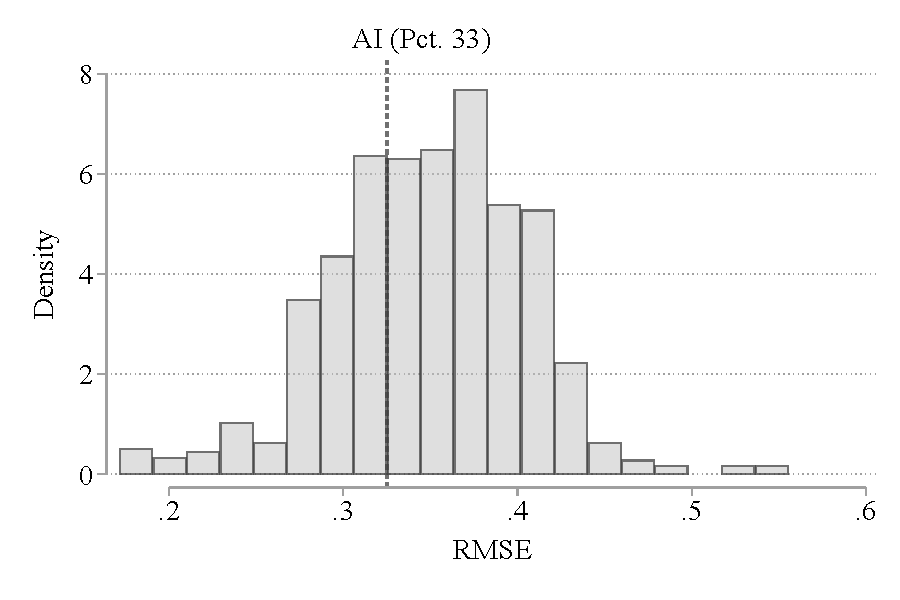
\includegraphics[width=7cm]{images/rmse_top_level_IN_NAI.pdf} }}%
    \qquad
    \subfloat[\centering AUROC Radiologists and AI]{{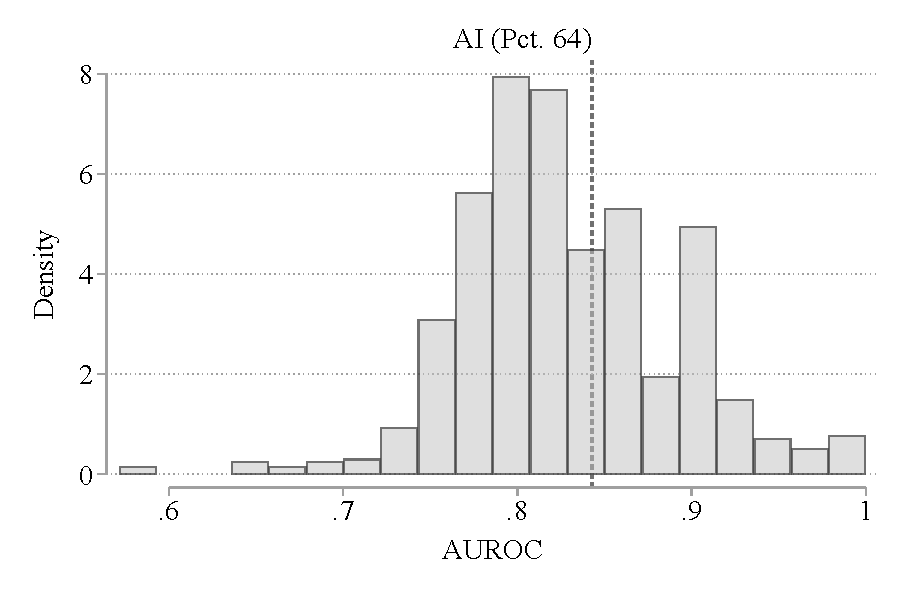
\includegraphics[width=7cm]{images/auroc_top_level_IN_NAI.pdf} }}%
\end{figure}
\begin{footnotesize}
  \noindent Note: These histograms show distributions of two different accuracy measures of radiologist assessments alongside the AI's accuracy. The left graph shows the distribution of the RMSE while the right shows the distribution of the average AUROC. Both distributions are shrunk to the grand mean using empircal Bayes. These measures are for each radiologist and include the top-level pathologies. The dotted line is the average measure of the AI algorithm for the corresponding distribution. Only the assessments where contextual history information is available for the radiologists but not the AI prediction are considered. 
\end{footnotesize}

\begin{figure}[H] 
\caption{AI Influence\label{fig:ai-influence}}
    \begin{center}
    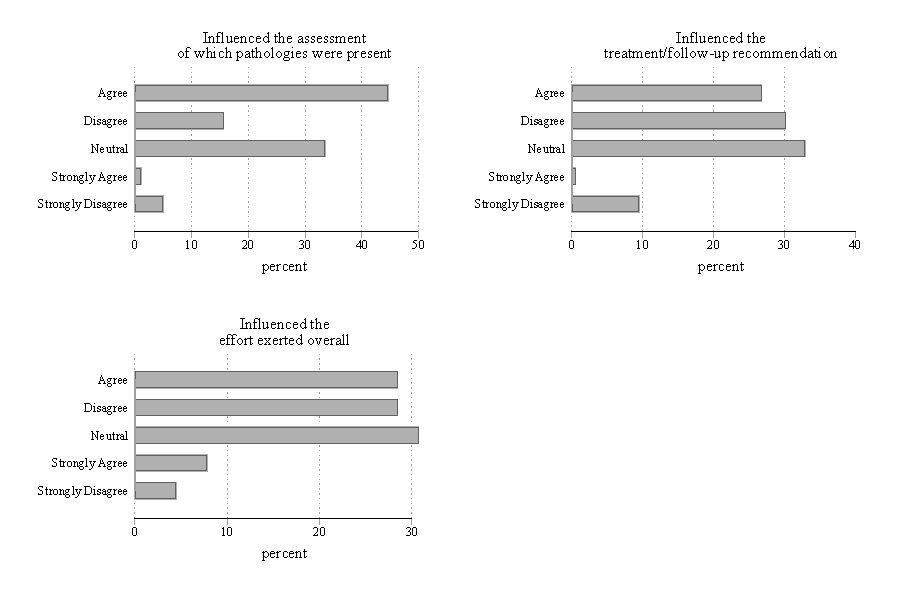
\includegraphics[width=0.8\textwidth]{images/ai_influence.pdf}
    \end{center}
\end{figure}

\begin{figure}[H]
    \caption{Clinical History Influence\label{fig:ch-influence}}
    \begin{center}
    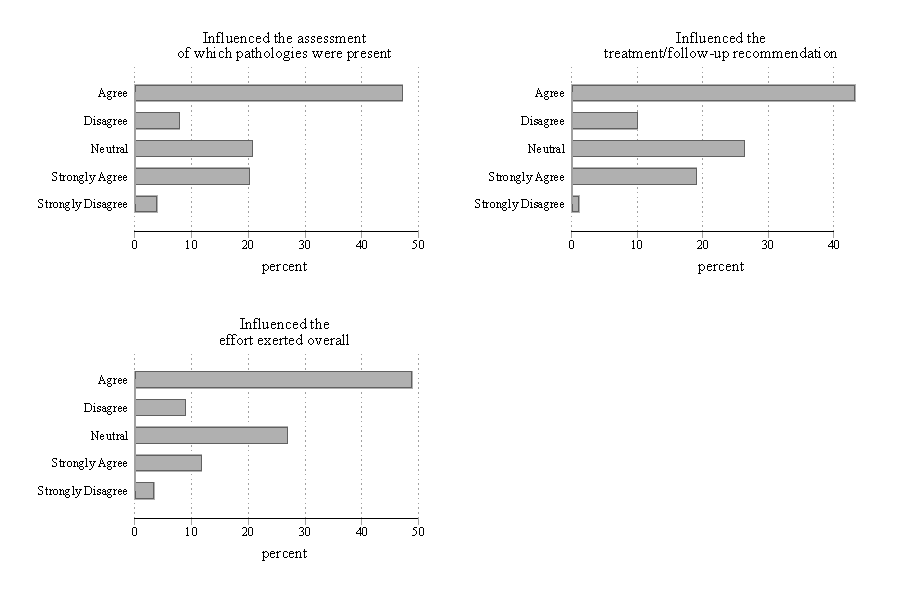
\includegraphics[width=0.8\textwidth]{images/ph_influence.pdf}
    \end{center}
\end{figure}

\clearpage

\subsection*{Appendix: Variables \label{subsec:Appendix:-Variables} }

\begin{table}[H]
\caption{Variable List}
%\begin{threeparttable}
\resizebox{\textwidth}{!}{%
\begin{tabular}{|l|l|l|l|}

\toprule[1pt]

Variable & Data Type & Range & Description \\
\hline
uid clean & str & & Radiologist identifier \\
design & dbl & ${1,2,3}$ & Design arm \\
patient id & str & & Patient identifier \\
pathology & str & & Pathology \\
round & long & $[1,100] \in N$ & Patient-case read sequence within radiologist-session \\
 & & & (minimum value is 1) \\
treat & int & ${0,1}$ & Indicator if radiologist selected treat/follow-up. \\
 & & &  Missing for pathologies where it was deemed not relevant \\
treatment & str & & Information environment under which case was read \\
level & int & ${0,1,2,3}$ & Position in pathology hierarchy (e.g. level 0 is top-level) \\
visible & int & ${0,1}$ & Indicator if pathology was visible when rad submitted case \\
probability & dbl & $[0,1]$ & Probability radiologist reported on interface slider \\
severity & str & & Response to severity question, when relevant \\
size & str & & Response to size question, when relevant\\
position & str & & Response to position question, when relevant \\
active time & dbl & & Time spent actively working on case (in seconds) \\
raw time & dbl & & Total time spent on case (in seconds) \\
num clicks & dbl & & Number of clicks on a case \\
group vietnam & int & ${0,1}$ & Indicator if the radiologist is from VinMac healthcare system, Vietnam \\
group teleradiology & int & ${0,1}$ & Indicator if the radiologist is from a tele radiology company \\
group pilot & int & ${0,1}$ & Indicator if the radiologist is from the experiment pilot \\
group ground truth & int & ${0,1}$ & Indicator if the radiologist is a ground truth radiologist \\
incentive round & int & ${0,1}$ & Indicator if incentives for correct diagnosis were provided \\
total num rounds & long & $[65,100]$ & The total number of reads by one radiologist  \\
chexbert label x & dbl & ${0,1}$ & ChexBert label for this case / pathology \\
ch indication & str & & Physician's indication for a given case \\
ch weight & str & & Weight(in lbs) of the patient under consideration \\
ch bp & str & & BP of the patient under consideration\\
ch temp & str & & Temperature of the patient under consideration \\
ch pulse & dbl & $[60,120]$ & Pulse of the patient under consideration \\
ch age & long & $[20,99]$ & Age of the patient under consideration \\
ch num labs & long & $[0,43]$ & Number of labels associated with a patient \\
ch num flagged labs & long & $[0,25]$ & Number of labels flagged as abnormal \\
ch gender & str & & Gender of the patient under consideration \\
alg pred & dbl & $[0,1]$ & AI prediction \\
with ai & byte & ${0,1}$ & Indicator if radiologist had access to AI \\
with ch & byte & ${0,1}$ & Indicator if radiologist had access to CH \\
gt average XX & dbl & $[0,1]$ & Average of ground truth probabilities for \\
 & & & group XX (us, vietnam, all, experiment) \\
gt average logodds XX & dbl & $[0,1]$ & Log-odds average (transformed into probability space) \\
 & & & probabilities for group XX \\
gt binary logodds XX & long & ${0,1}$ & Binary ground truth based on LO average for group XX \\
gt binary simple XX & long & ${0,1}$ & Binary ground truth based on simple average for group XX \\
gt treat XX & long & ${0,1}$ & Majority GT radiologists saying treat / follow-up for group XX \\
gt treat sum XX & dbl & ${0,1,2,3,4}$ & Number of GT radiologists saying treat / follow-up for group XX \\
gt average active time XX & dbl & $(35,344)$ & Average active time of the GT radiologists \\
ground truth & dbl & $[0,1]$ & Ground truth passed as an argument \\
ground truth treat & dbl & $[0,1]$ & Treatment ground truth, for group passed as argument \\
experiment id & str & & Radiologist identifier \\
experiment session & int & ${0,1,2,3}$ & Session number \\
case average active time & dbl & $[50,335]$ & Average time spent on a case by the radiologist \\
alg pred calibrated & dbl & $[0,1]$ & Calibrated version of the AI \\

\bottomrule[1pt]
\end{tabular}%
}
%\end{threeparttable}
\end{table}

\clearpage

\subsection*{Appendix: Experiment Interface \label{subsec:Appendix:-Experiment-Interface}}

The experimental interface was created with the intention to mimic
clinical practice while generating quantitative inputs for analysis.
Following is the information that the radiologists received before
starting the experiment. Comments on the instructions are provided
in italics and were not seen by subjects.

\subsubsection*{Section 1: Instructions}

You are about to participate in a study on medical decision making.
You may pause the study at any time. To resume, revisit the link you
were given and your progress will have been saved.

We will present you with adult patients with potential thoracic pathologies.
These patients will be presented under the following four scenarios:
\begin{enumerate}
\item Only a chest X-ray is shown.
\item An X-ray is accompanied with additional information about the \uline{clinical
history.}
\item An X-ray is shown along with \uline{Artificial Intelligence (AI)
support}. This AI tool is described in further detail below.
\item An X-ray is shown along with both additional information on \uline{clinical
history} and the \uline{AI support.}
\end{enumerate}
%
The patients are randomly assigned to each of these scenarios. That
is, availability of \uline{clinical history} and/or \uline{AI
support} is unrelated to the patient.

\uline{Clinical History:} includes available lab results or indications
by the treating physician, if any.

\uline{AI support:} This tool uses only the X-ray image to predict
the probability of each potential pathology of interest. The tool
is based on state-of-the-art machine learning algorithms developed
by a leading team of researchers at Stanford University.

\textbf{Responses}

For each patient and pathology, we will ask for both an assessment
and a treatment decision:
\begin{enumerate}
\item We will first ask for your assessment of the probability that each
condition is present in a patient. \textbf{Please consider all pathologies
and findings that would be relevant in a radiology report for the
patient. You should express your uncertainty about the presence of
one or many conditions by appropriately choosing the probability.}
Note that it is possible that the patient has multiple such conditions
or none of them.
\item If you determine that a pathology may be present, we may ask you to
rate the severity and/or extent of the disease on a scale.
\item Finally, when relevant we will ask whether you would recommend treatment
or follow up according to the clinical standard of care if you determine
that the pathology may be present. The first two responses are diagnostic
while the third is a clinical decision. We are aware that a single
physician or radiologist typically does not perform both tasks. However,
for this study, we ask that you respond to the best of your ability
in both of these roles.
\end{enumerate}
\textbf{Browser Compatibility}

This platform supports desktop versions of Chrome, Firefox, and Edge.
Important features on non-supported browsers (including Safari) are
missing and we discourage their use for this experiment. In addition,
the platform does not support any mobile devices and the platform
will perform poorly on mobile. If you encounter any issues during
the experiment, please send an email to \href{mailto:DiagnosticAI@mit.edu}{DiagnosticAI@mit.edu}
and we will follow-up quickly.

\subsubsection*{Section 2: Clinical Hierarchy}

The interface uses a hierarchy to categorize various thoracic conditions.
It will be useful to familiarize yourself with this hierarchy before
you start, but you may also revisit the hierarchy at any time throughout
the experiment by clicking the help tab in the upper right corner.\textit{
{[}The probability for the sub-pathologies is required only if the
parent pathology prevalence is greater than 10\%{]}}

\begin{figure}[H]
\caption{Pathology Hierarchy}

\begin{center}
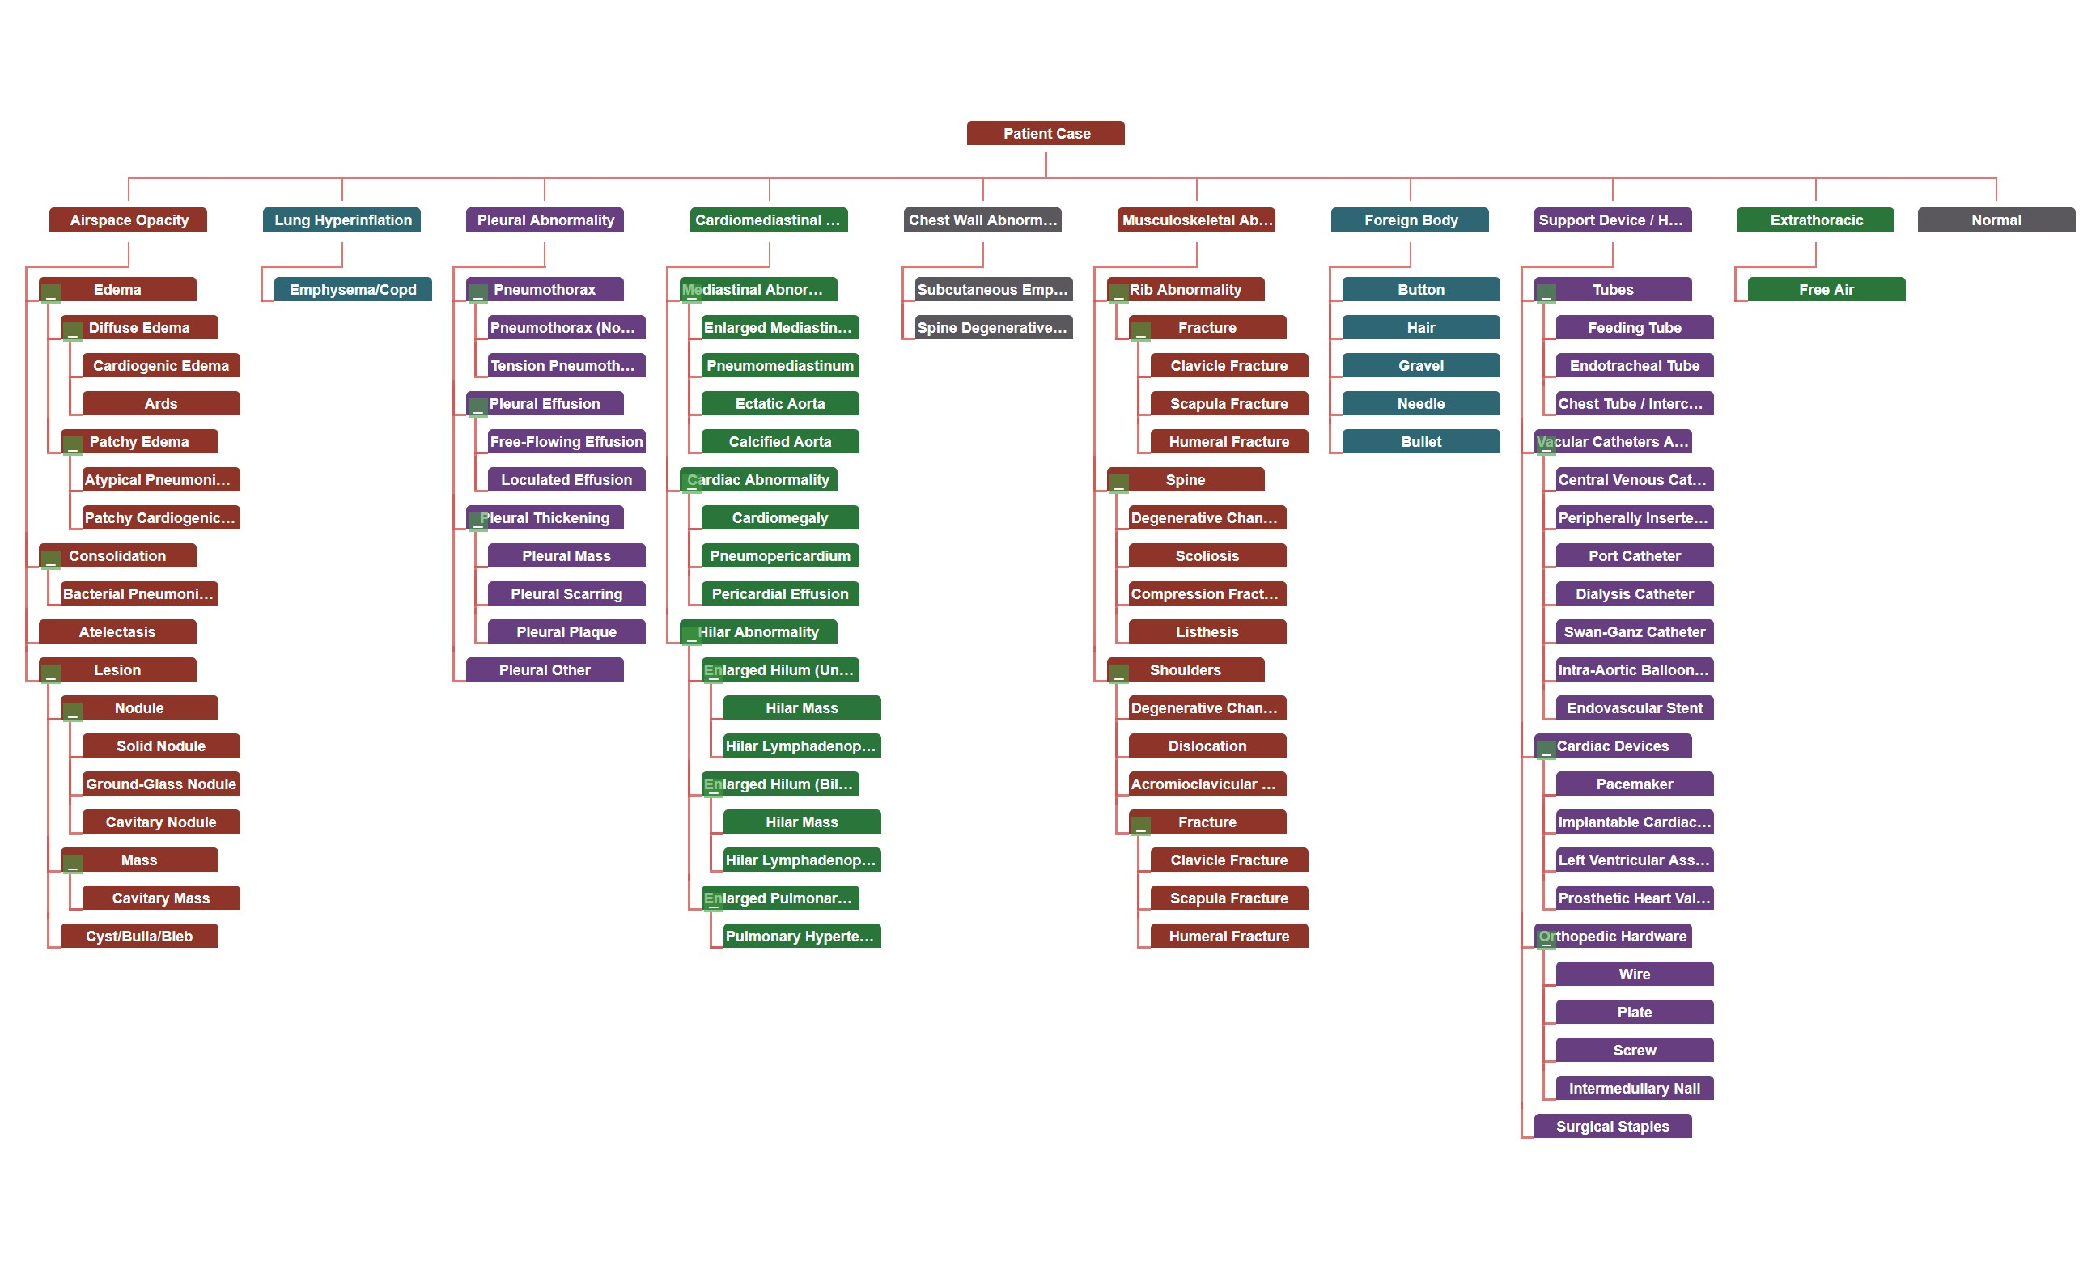
\includegraphics[width=1\textwidth]{images/pat_hierarchy.pdf}
\end{center}
\end{figure}


\subsubsection*{Section 3: AI Support Tool}

The AI support tool that is provided uses only the X-ray image to
predict the probability of each potential pathology of interest. The
tool is based on state-of-the-art machine learning algorithms developed
by a leading team of researchers at Stanford University. The tool
is trained only on X-ray images, meaning it does not incorporate the
clinical history of the patients.

\textbf{Performance of the AI Support}

The AI tool is described in \href{https://arxiv.org/abs/1901.07031}{Irvin et al. [2019]},
which showed the AI tool performed at or near expert levels across
the pathologies studied. Below we plot two measures of performance
of the AI tool. We plot in blue the accuracy of the tool, defined
as the share of cases correctly diagnosed when treating false positives
and false negatives equally. In red, we plot the Area Under the ROC
curve (AUC), which is another measure of AI classification performance.
The AUC is a number between 0 and 100\%, with numbers close to 100\%
representing better algorithm performance. The AUC is equal to the
probability that a randomly chosen positive case is ranked higher
than a randomly chosen negative case.

\begin{figure}[H]
\caption{Performance of AI Tool}

\begin{center}
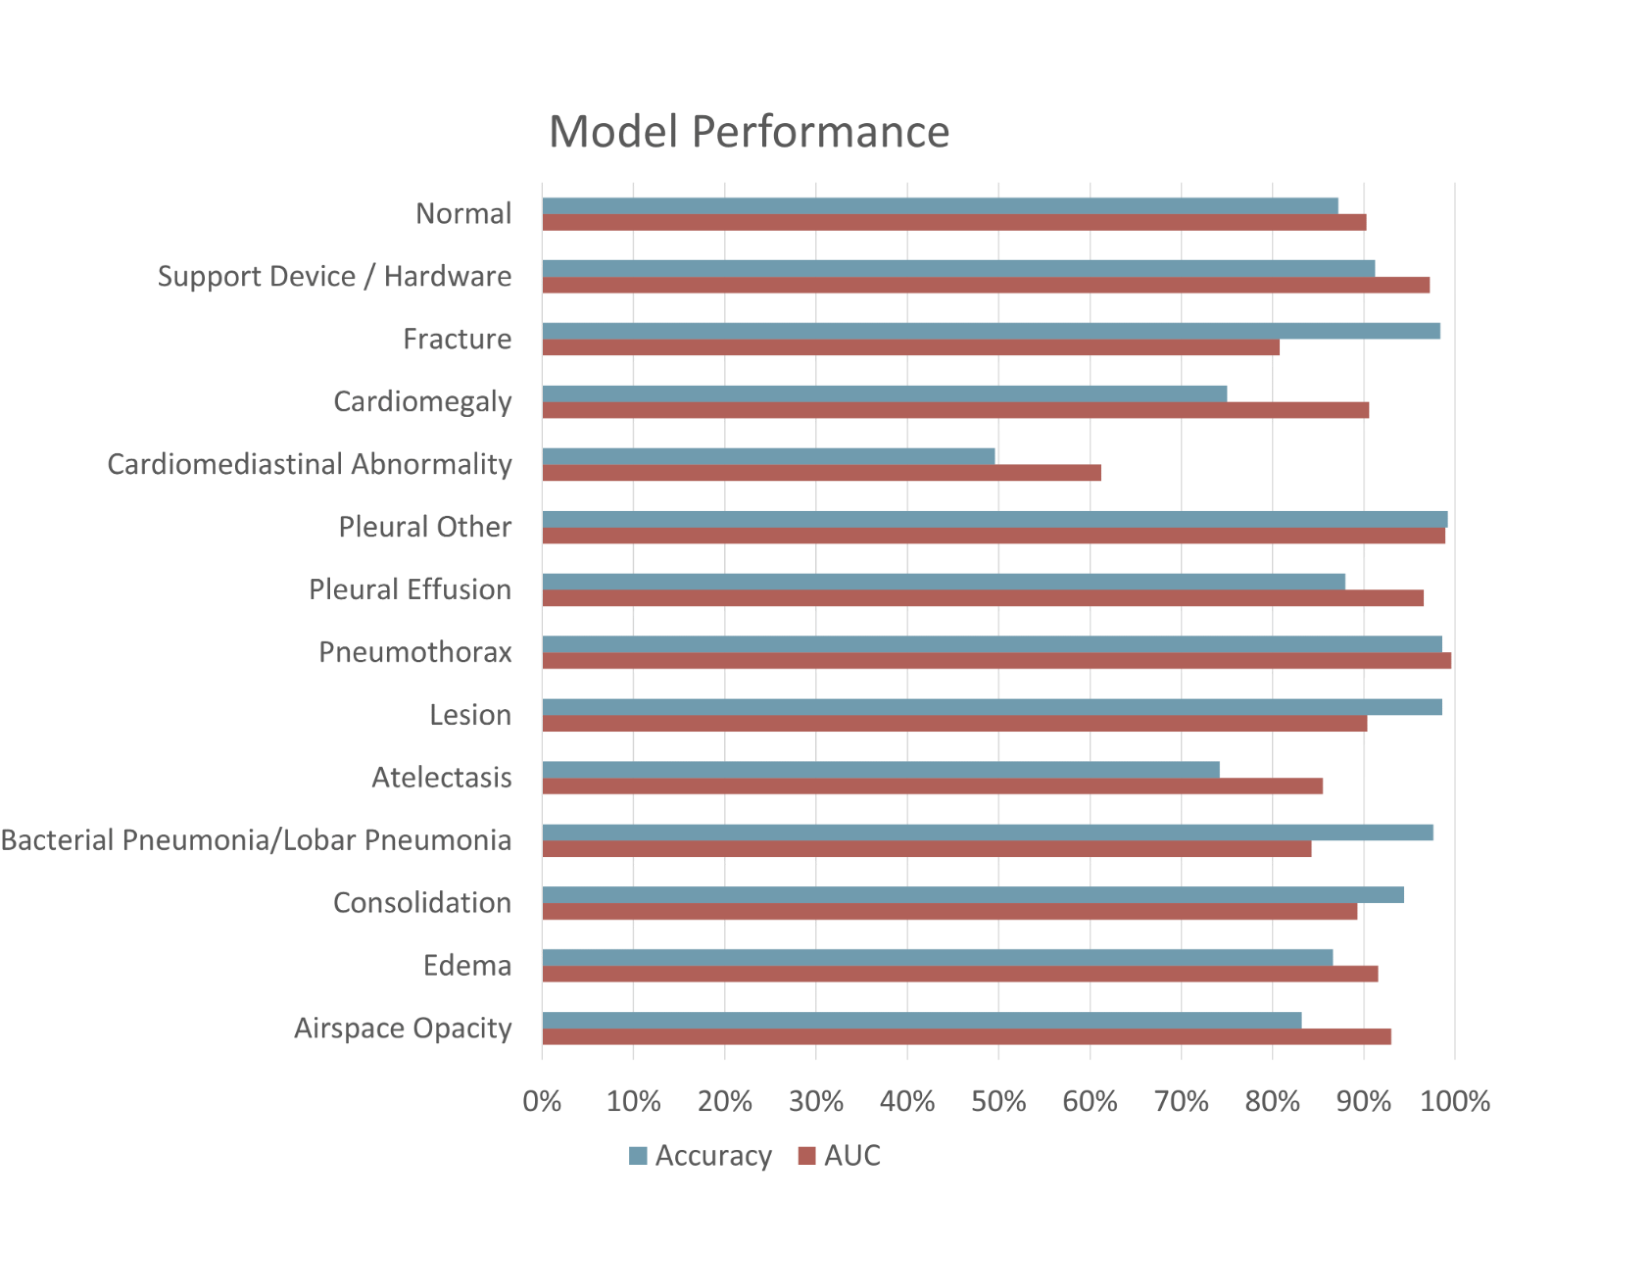
\includegraphics[scale=0.6]{images/ai_instruction_accuracy.pdf}
\end{center}
\end{figure}

\textbf{Example Images}

Below are 50 example images with the associated AI tool predictions.
These images are randomly chosen to allow you to familiarize yourself
with the AI support tool and its accuracy \emph{{[}Here we only provide
two out of the fifty images{]}.}

\begin{figure}[H]
\caption{Example Images}

\begin{center}
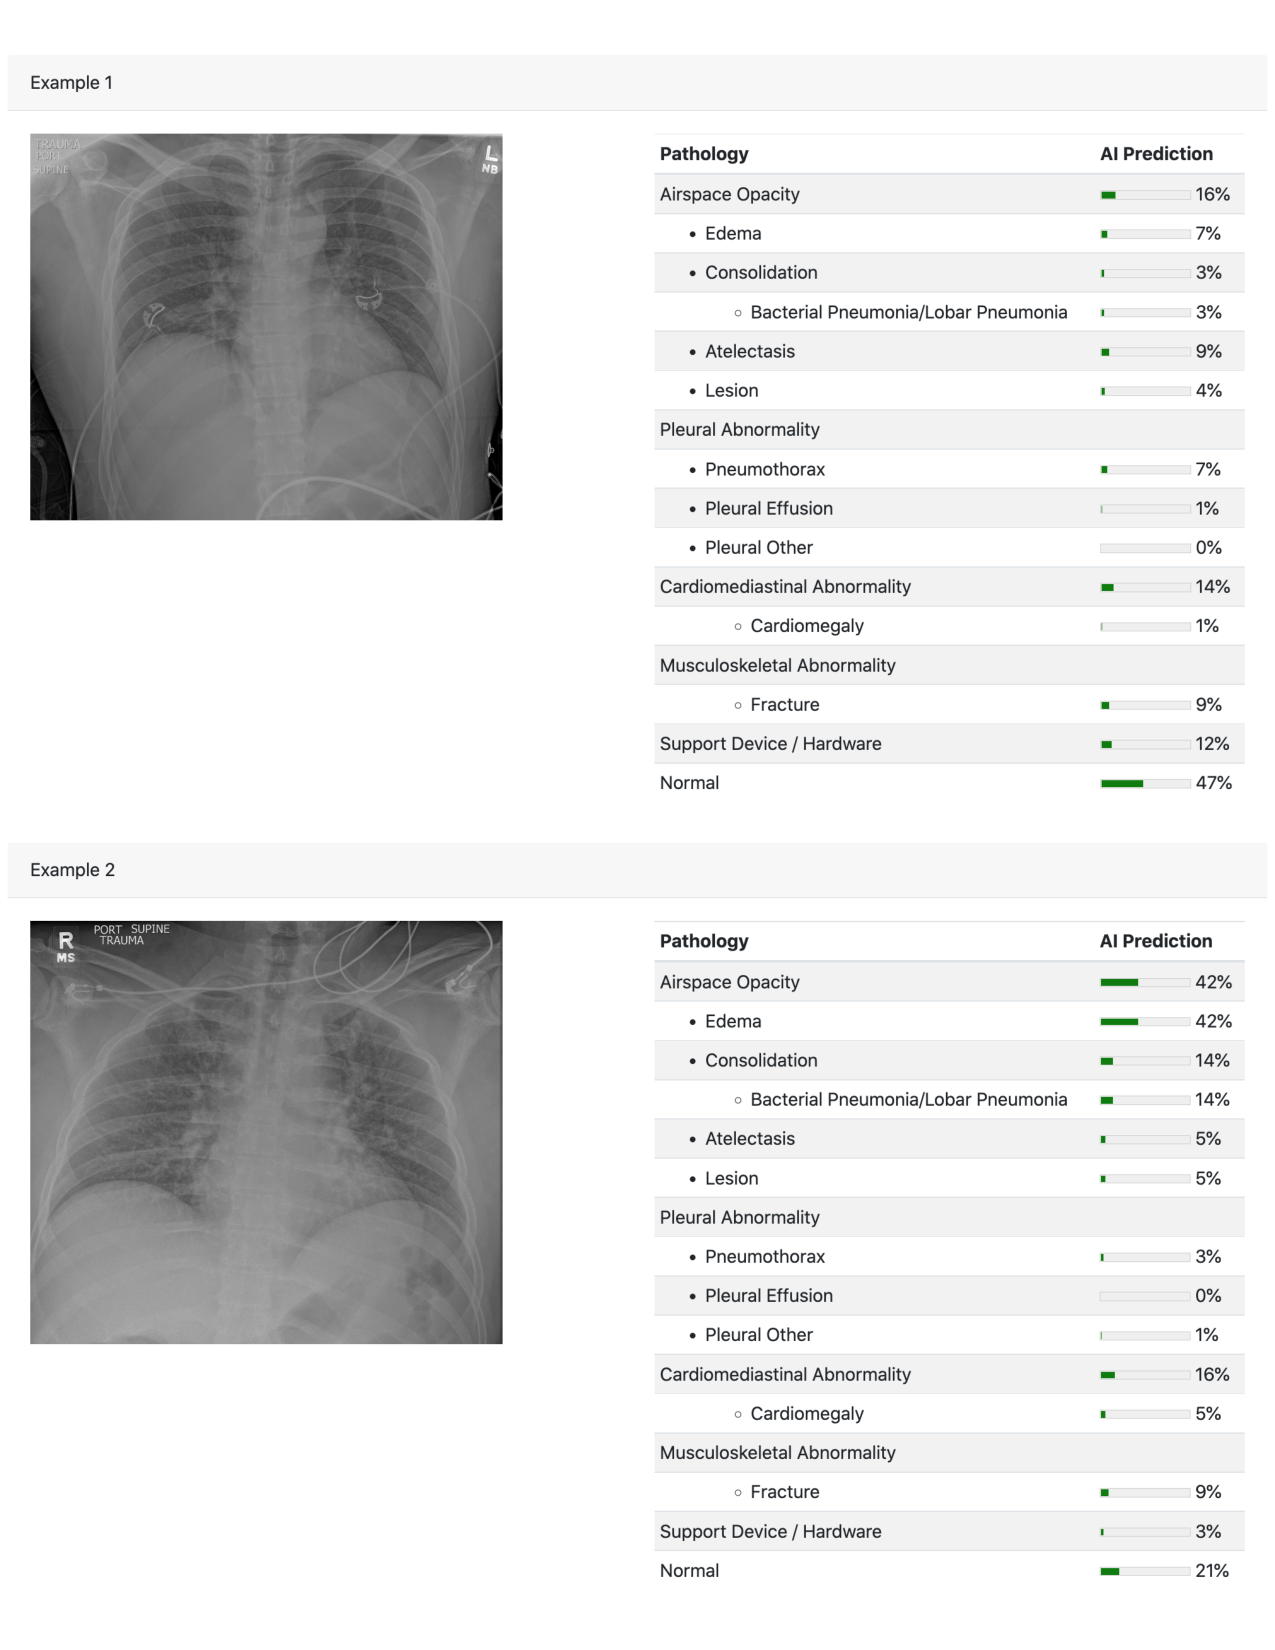
\includegraphics[scale=0.8]{images/ai_instruction_example.pdf}
\end{center}
\end{figure}
\textbf{Section 4: Demonstration}

The brief video below walks you through the interface and a few examples.
\emph{{[}At this stage participants saw an instruction video which
can be founds \href{https://www.dropbox.com/s/fgdcokweekpm44r/RadExperimentV4.mp4?raw=1}{here}{]}}

\subsubsection*{Section 5: Consent I}

You have been asked to participate in a study conducted by researchers
from the Massachusetts Institute of Technology (M.I.T.) and Harvard
University.

The information below provides a summary of the research. Your participation
in this research is voluntary and you can withdraw at any time.
\begin{enumerate}
\item Study procedure: We will ask you to examine a number of chest x-rays.
We will vary both the amount of information provided about the patient
and the availability of an AI support tool.
\item Potential Risks \& Benefits: There are no foreseeable risks associated
with this study and you will receive no direct benefit from participating.
\end{enumerate}
%
Your participation in this study is completely voluntary and you are
free to choose whether to be in it or not. If you choose to be in
this study, you may subsequently withdraw from it at any time without
penalty or consequences of any kind. The investigator may withdraw
you from this research if circumstances arise.

\subsubsection*{Section 6: Consent II}

\textbf{Privacy \& Confidentiality}

The only people who will know that you are a research subject are
members of the research team which might include outside collaborators
not affiliated with MIT. No identifiable information about you, or
provided by you during the research, will be disclosed to others without
your written permission, except: if necessary to protect your rights
or welfare, or if required by law. In addition, your information may
be reviewed by authorized MIT representatives to ensure compliance
with MIT policies and procedures.

When the results of the research are published or discussed in conferences,
no information will be included that would reveal your identity.

\textbf{Questions}

If you have any questions or concerns about the research, please feel
free to contact us directly at diagnosticAI@mit.edu.

\textbf{Your Rights}

You are not waiving any legal claims, rights or remedies because of
your participation in this research study. If you feel you have been
treated unfairly, or you have questions regarding your rights as a
research subject, you may contact the Chairman of the Committee on
the Use of Humans as Experimental Subjects, M.I.T., Room E25-143B,
77 Massachusetts Ave, Cambridge, MA 02139, phone 1-617-253 6787.

I understand the procedures described above. By clicking next, I am
acknowledging my questions have been answered to my satisfaction,
and I agree to participate in this study.

\subsubsection*{Section 7: Interface questions}

\emph{{[}Each of these questions has a true of false response which
was entered through a radio button. Participants are not able to start
the experiment without answering each question correctly.{]}}

Before beginning the experiment, we would like to confirm a few facts
through the following comprehension questions. Please answer True
or False to the following questions.

1) The algorithm's prediction is based on information from both the
X-ray scan as well as the clinical history.

2) When the algorithm does not show a prediction, it is because the
algorithm thinks the pathology is not present.

3) The follow up decision refers to any treatment or additional diagnostic
procedures that one would conduct based on the findings of the report.

4) Two patients with the same probability score for a condition ought
to always receive the same \textquotedblleft follow-up\textquotedblright{}
recommendation.

5) When a condition at a higher level of the hierarchy receives a
less than ten percent chance of being present then all the lower level
conditions within this branch automatically receive a zero probability
of being present.

6) If the algorithm says that the probability of a pathology is present
with 80\% probability, it means that the AI predicts 80 cases out
of 100 have the pathology present.

7) Suppose your assessment is that the patient definitely has either
edema or consolidation, and you believe that edema is twice as likely
as consolidation. Then you would assign 66.67\% to edema and 33.33\%
to consolidation:

8) I should only indicate pathologies and findings that would be relevant
in a radiology report for the patient.

\subsubsection*{Section 8: Bonus (Randomized only for designs 1 and 3)}

Bonus Payment Thank you again for participating in our study. If your
responses in this section are close to the average response of an
independent group of radiologists for each case, we will give you
a \$120 gift card to a large e-commerce retailer of your choice (e.g.
Amazon, Flipkart). This payment rule is designed so that your chances
of winning the prize is highest if you report your best estimate of
the probability that the pathology is present. The precise payment
rule is available on request, and we will follow up after the experiment
if you win the gift card.

\subsubsection*{Section 9: Practice Images}

First, we will present you with 8 patients (Design 1) to practice
and familiarize yourself with the interface. In the practice you will
see 2 patient cases under each of the possible combinations of AI
support and clinical history availability. You will be compensated
for these reads even though they are just for practice. {[}\textit{5
practice images for design 1 and none for design 3}{]}

\subsubsection*{Section 10: Randomized Information Scenario }

{[}\textit{This is the start of the experiment. The dataset contains
only these observations and excludes any practice images data.}{]}

The extent of clinical history information provided is not homogenous.
The thoroughness of the information varies across available information
for every patient. Some examples of varying clinical history information
are: 




\end{document}